\chapter{Results}

\section{Detector}

\subsection{Electron Calibration}

\begin{figure}[H]
  \centering
  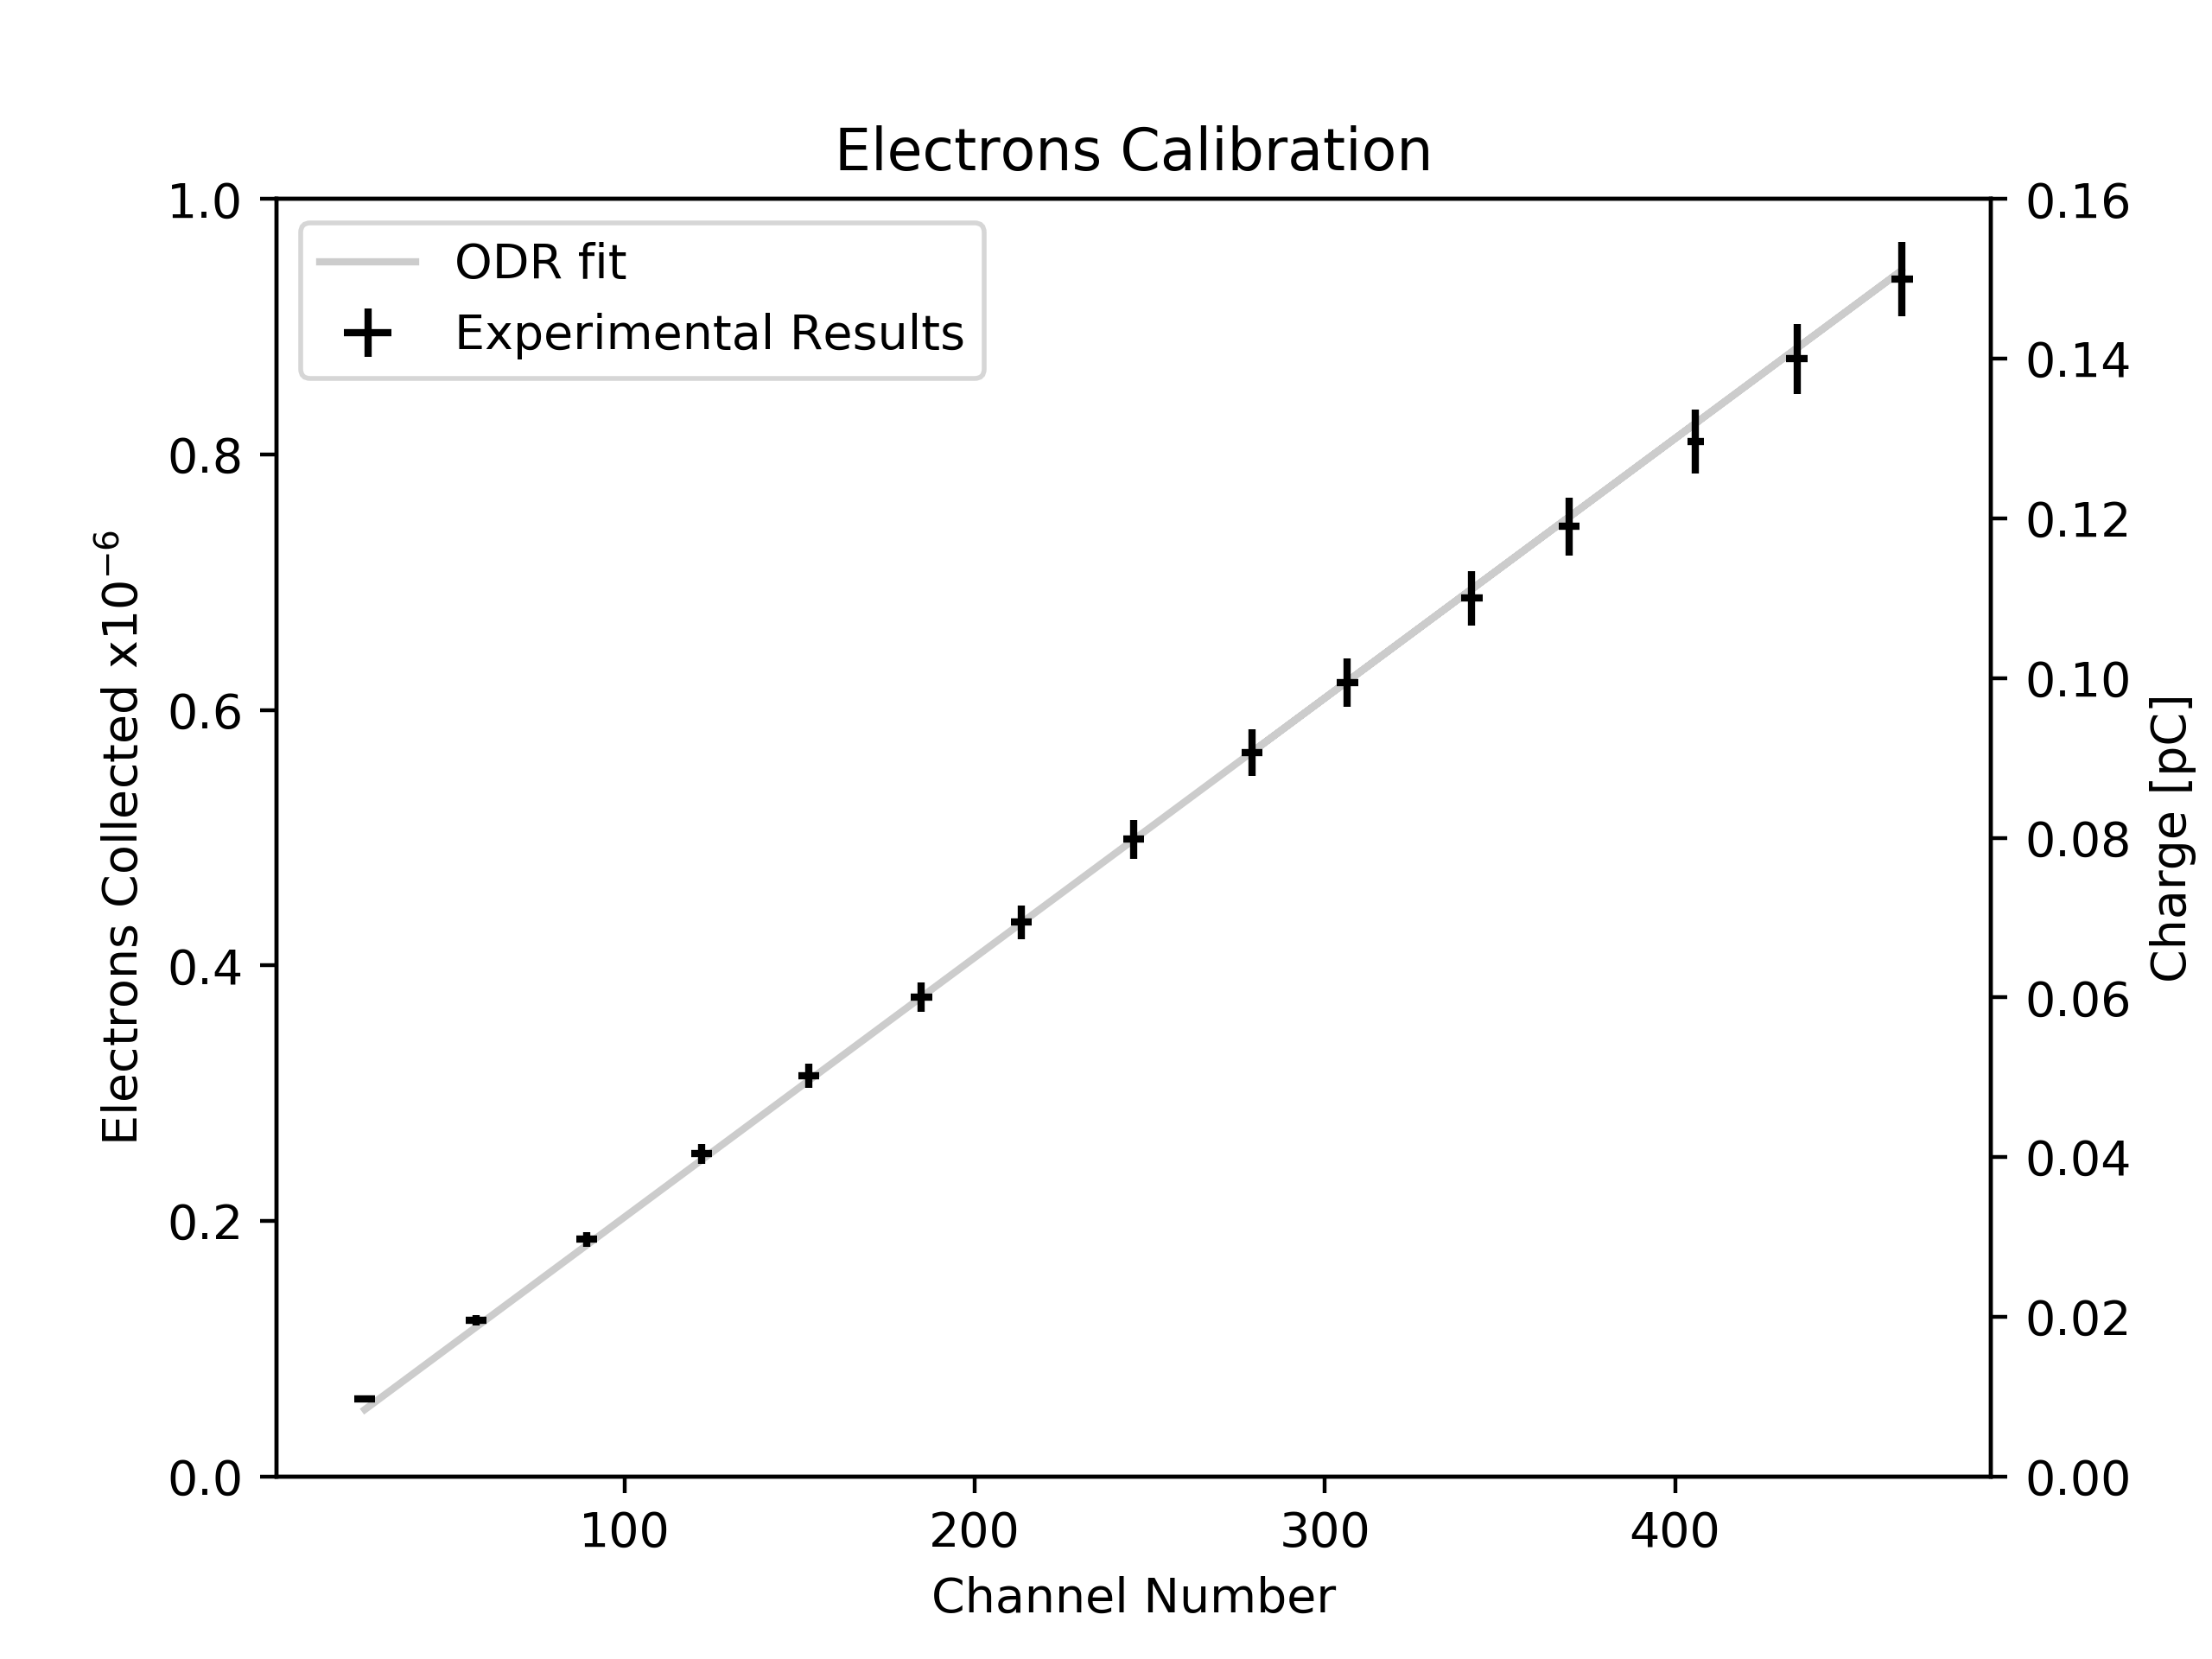
\includegraphics[width=\linewidth]{electronCalibration.png}
  \caption{Graph showing the relationship between MCA channel and the number of collected electrons. The line equation of the best fit line was $n_{e} = (2030\pm20)Ch$. Fitting a model with a constant term gave a line equation of $n_{e} = (1990\pm30)Ch + (8000\pm5000)$ which has a higher uncertainty.}
  \label{fig:calibration}
\end{figure}

\subsection{Voltage Run}

\begin{figure}[H]
  \centering
  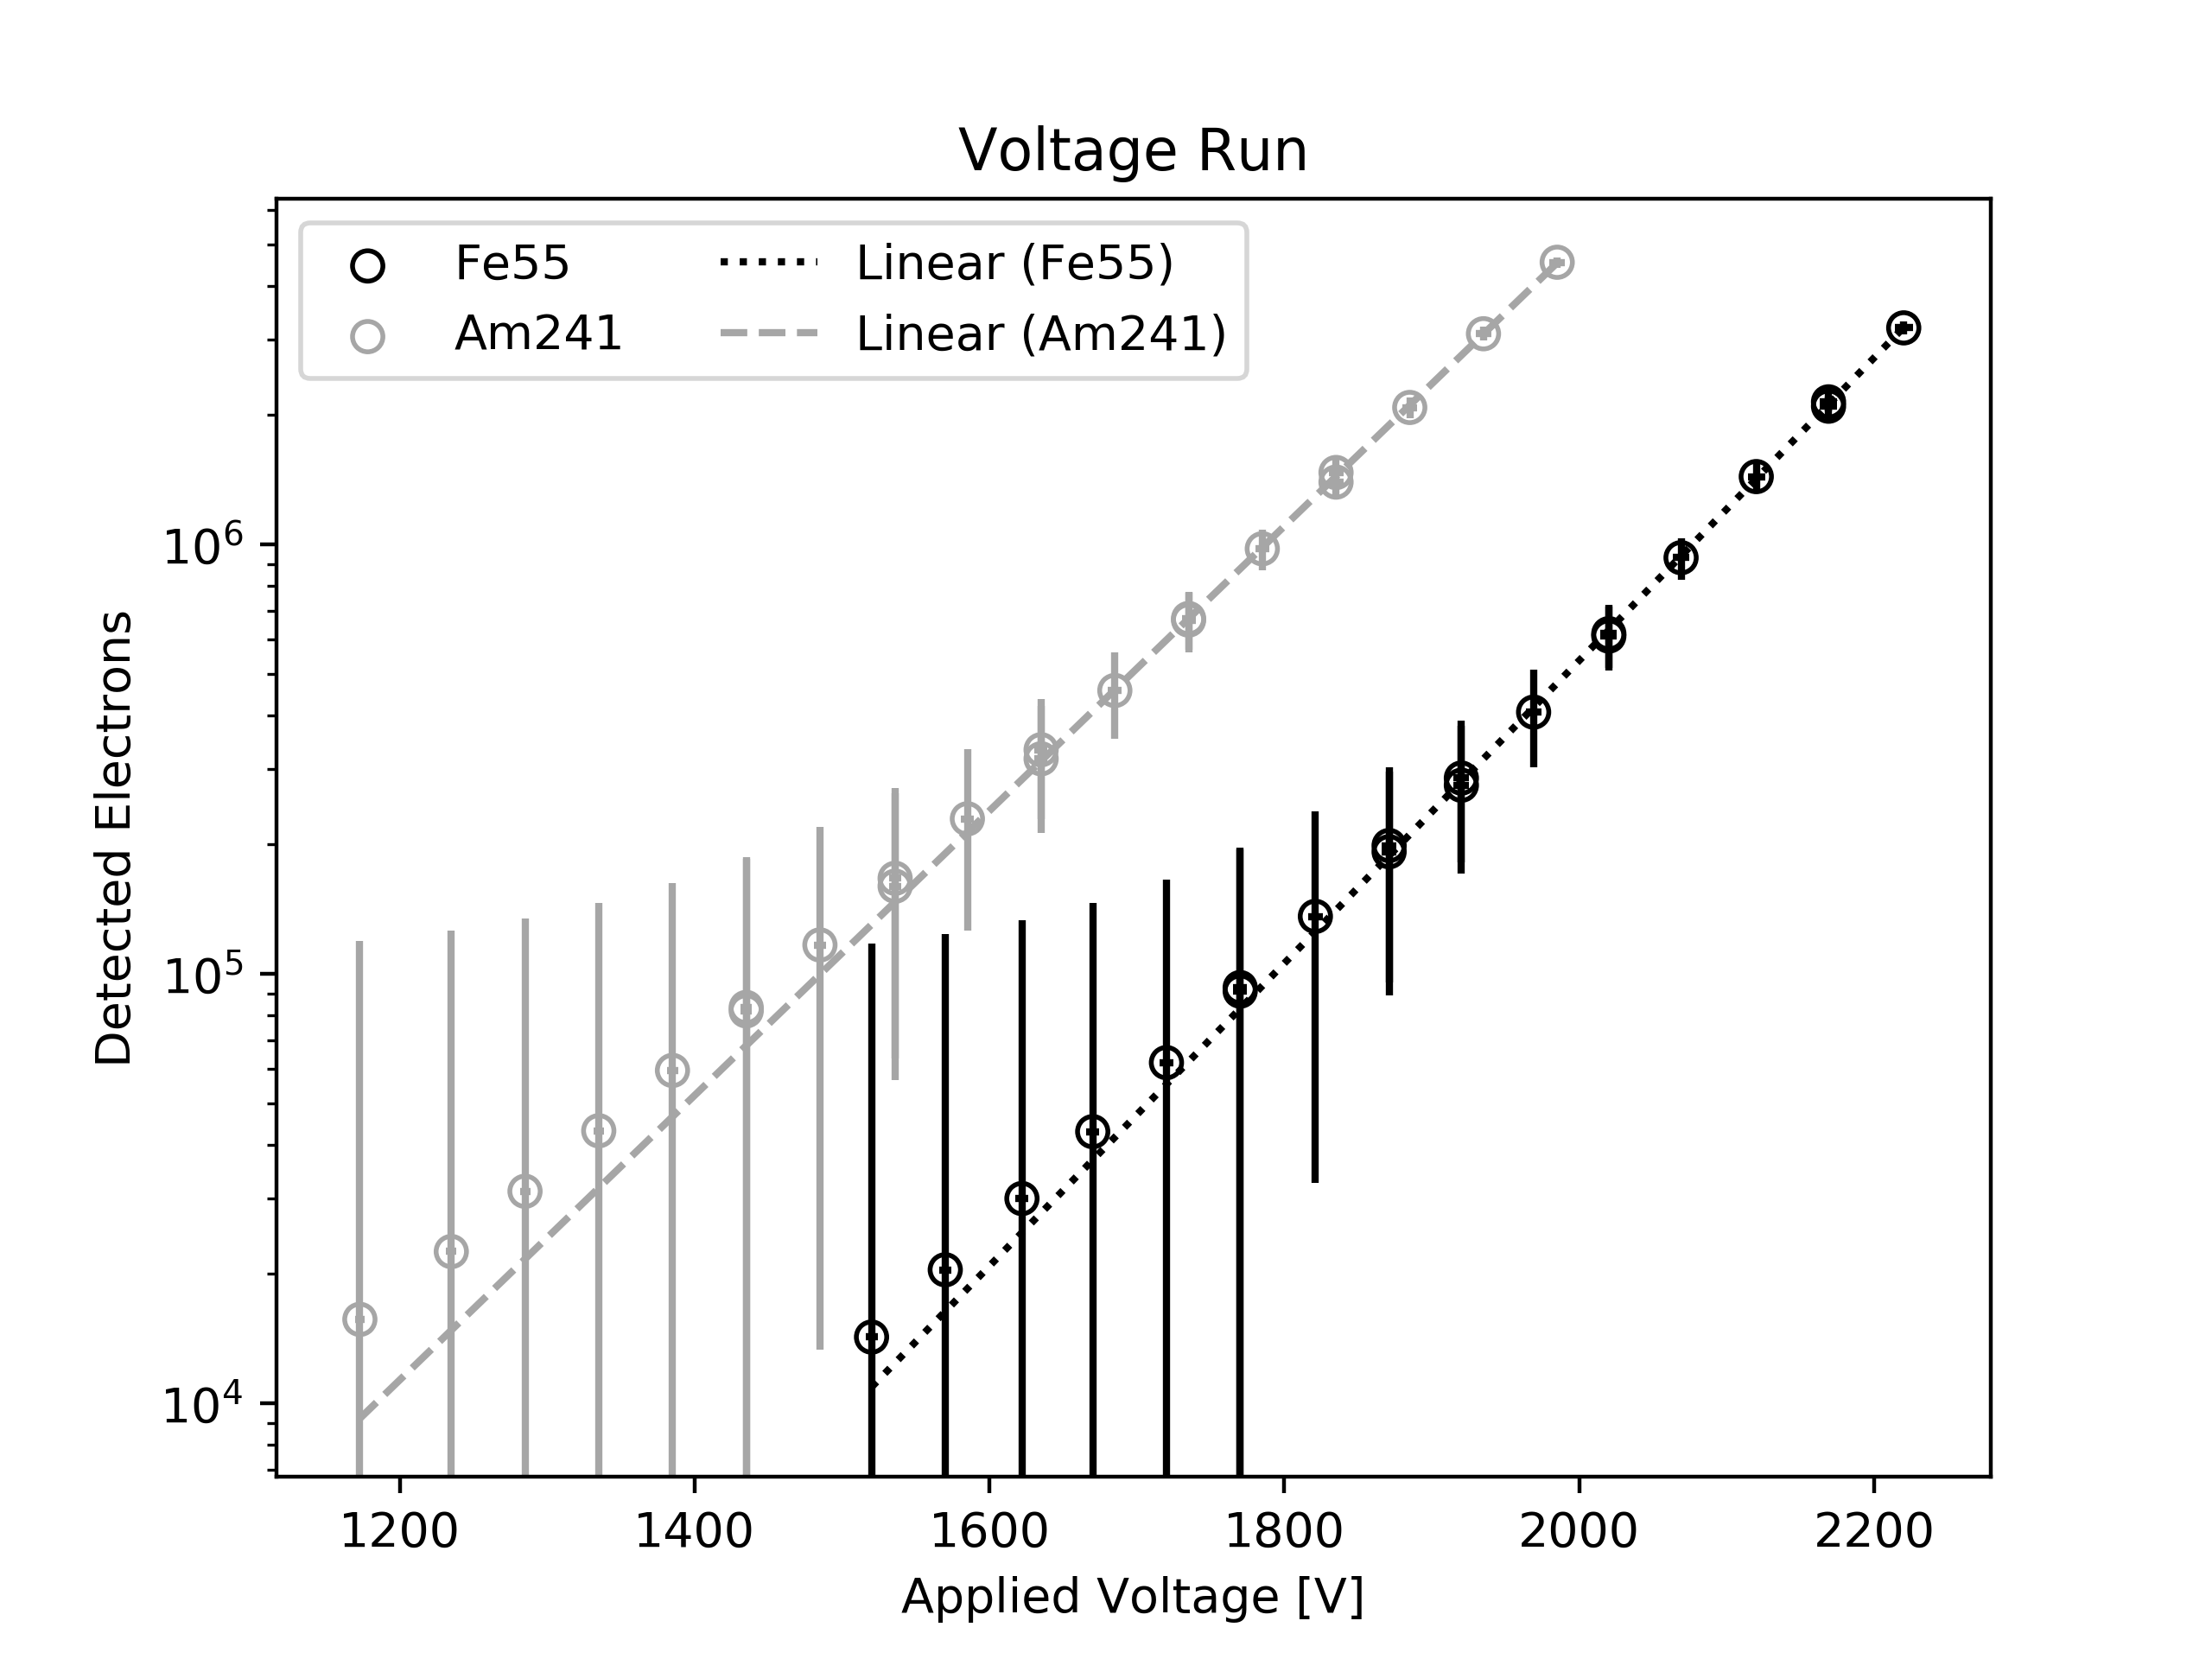
\includegraphics[width=11cm]{voltageRun.png}
  \caption{Results of the voltage run. The distribution for \textsuperscript{55}Fe and \textsuperscript{241}Am can be fitted by exponential functions: $n_{e}(Fe) = (0.05\pm0.04)\cdot\exp{(0.0081\pm0.0004)}$; $n_{e}(Am) = (1.2\pm0.6)\cdot\exp{(0.0076\pm0.0002)}$}
  \label{fig:voltageRun}
\end{figure}

\subsection{Multiplication Factor}

\begin{figure}[H]
  \centering
  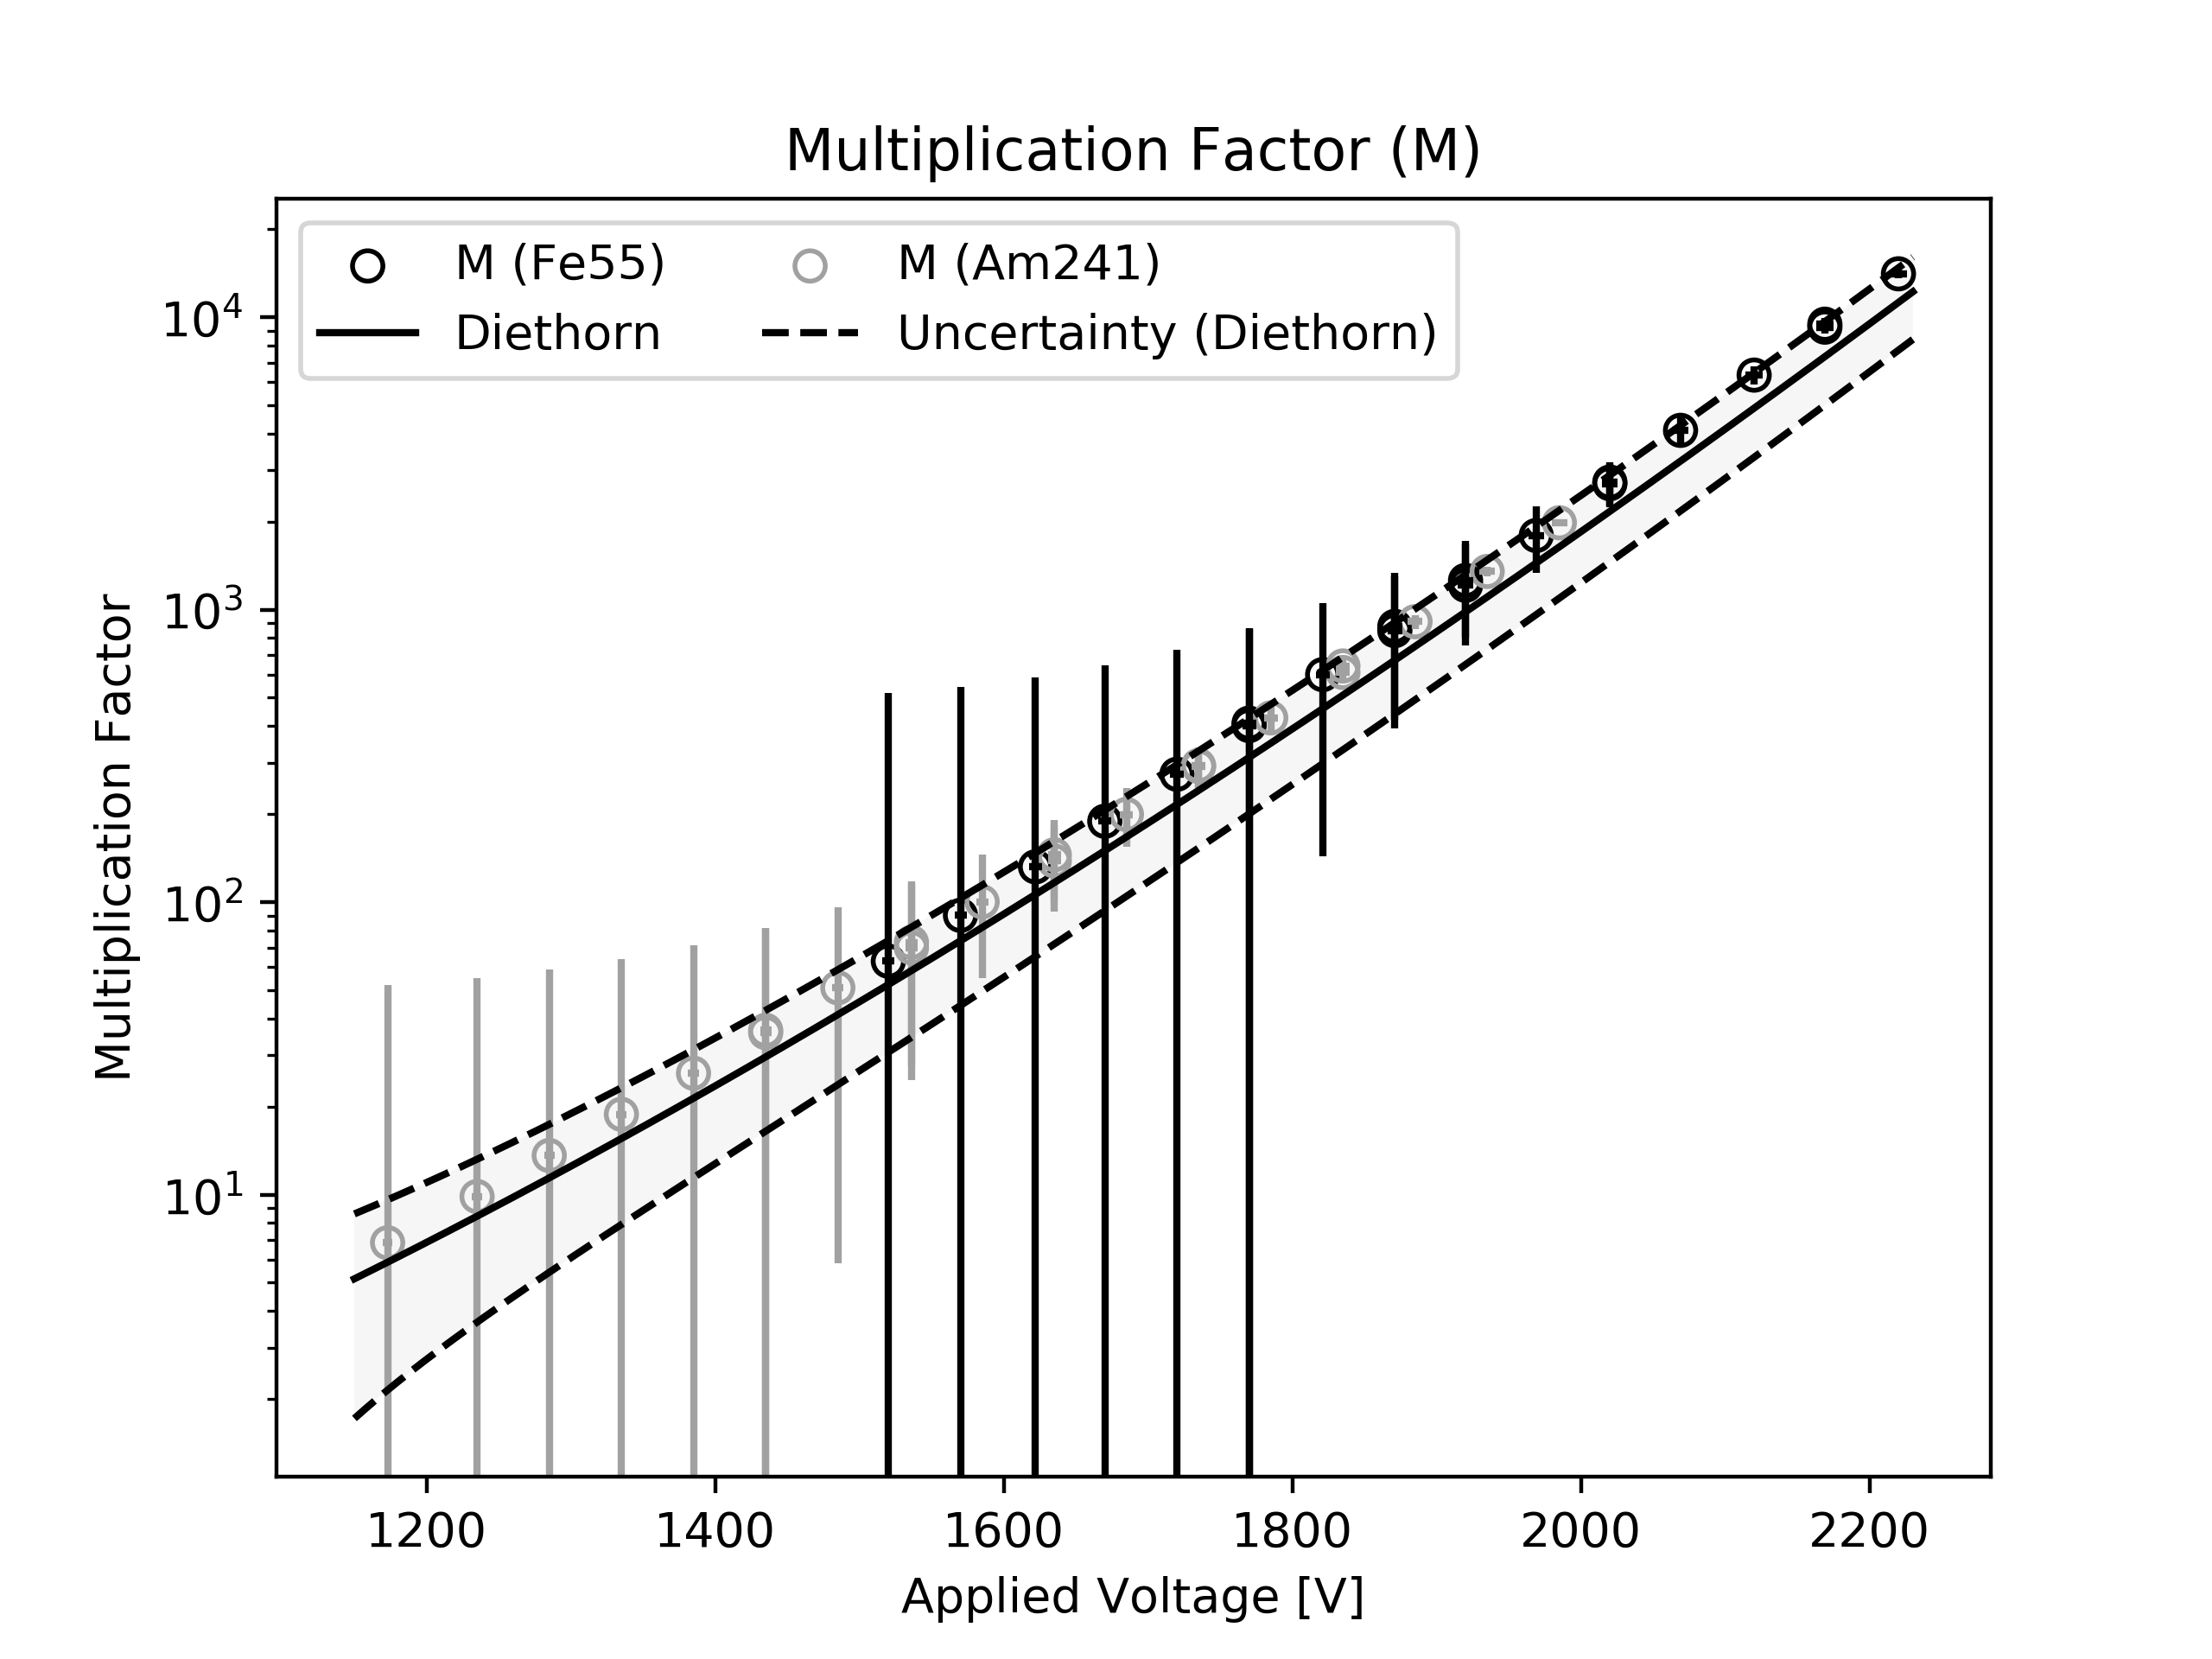
\includegraphics[width=11cm]{mFactor.png}
  \caption{Comparison of measured multiplication factor with the theoretical Diethorn formula.}
  \label{fig:mFactor}
\end{figure}

\subsection{Energy Resolution}

\begin{figure}[H]
  \centering
  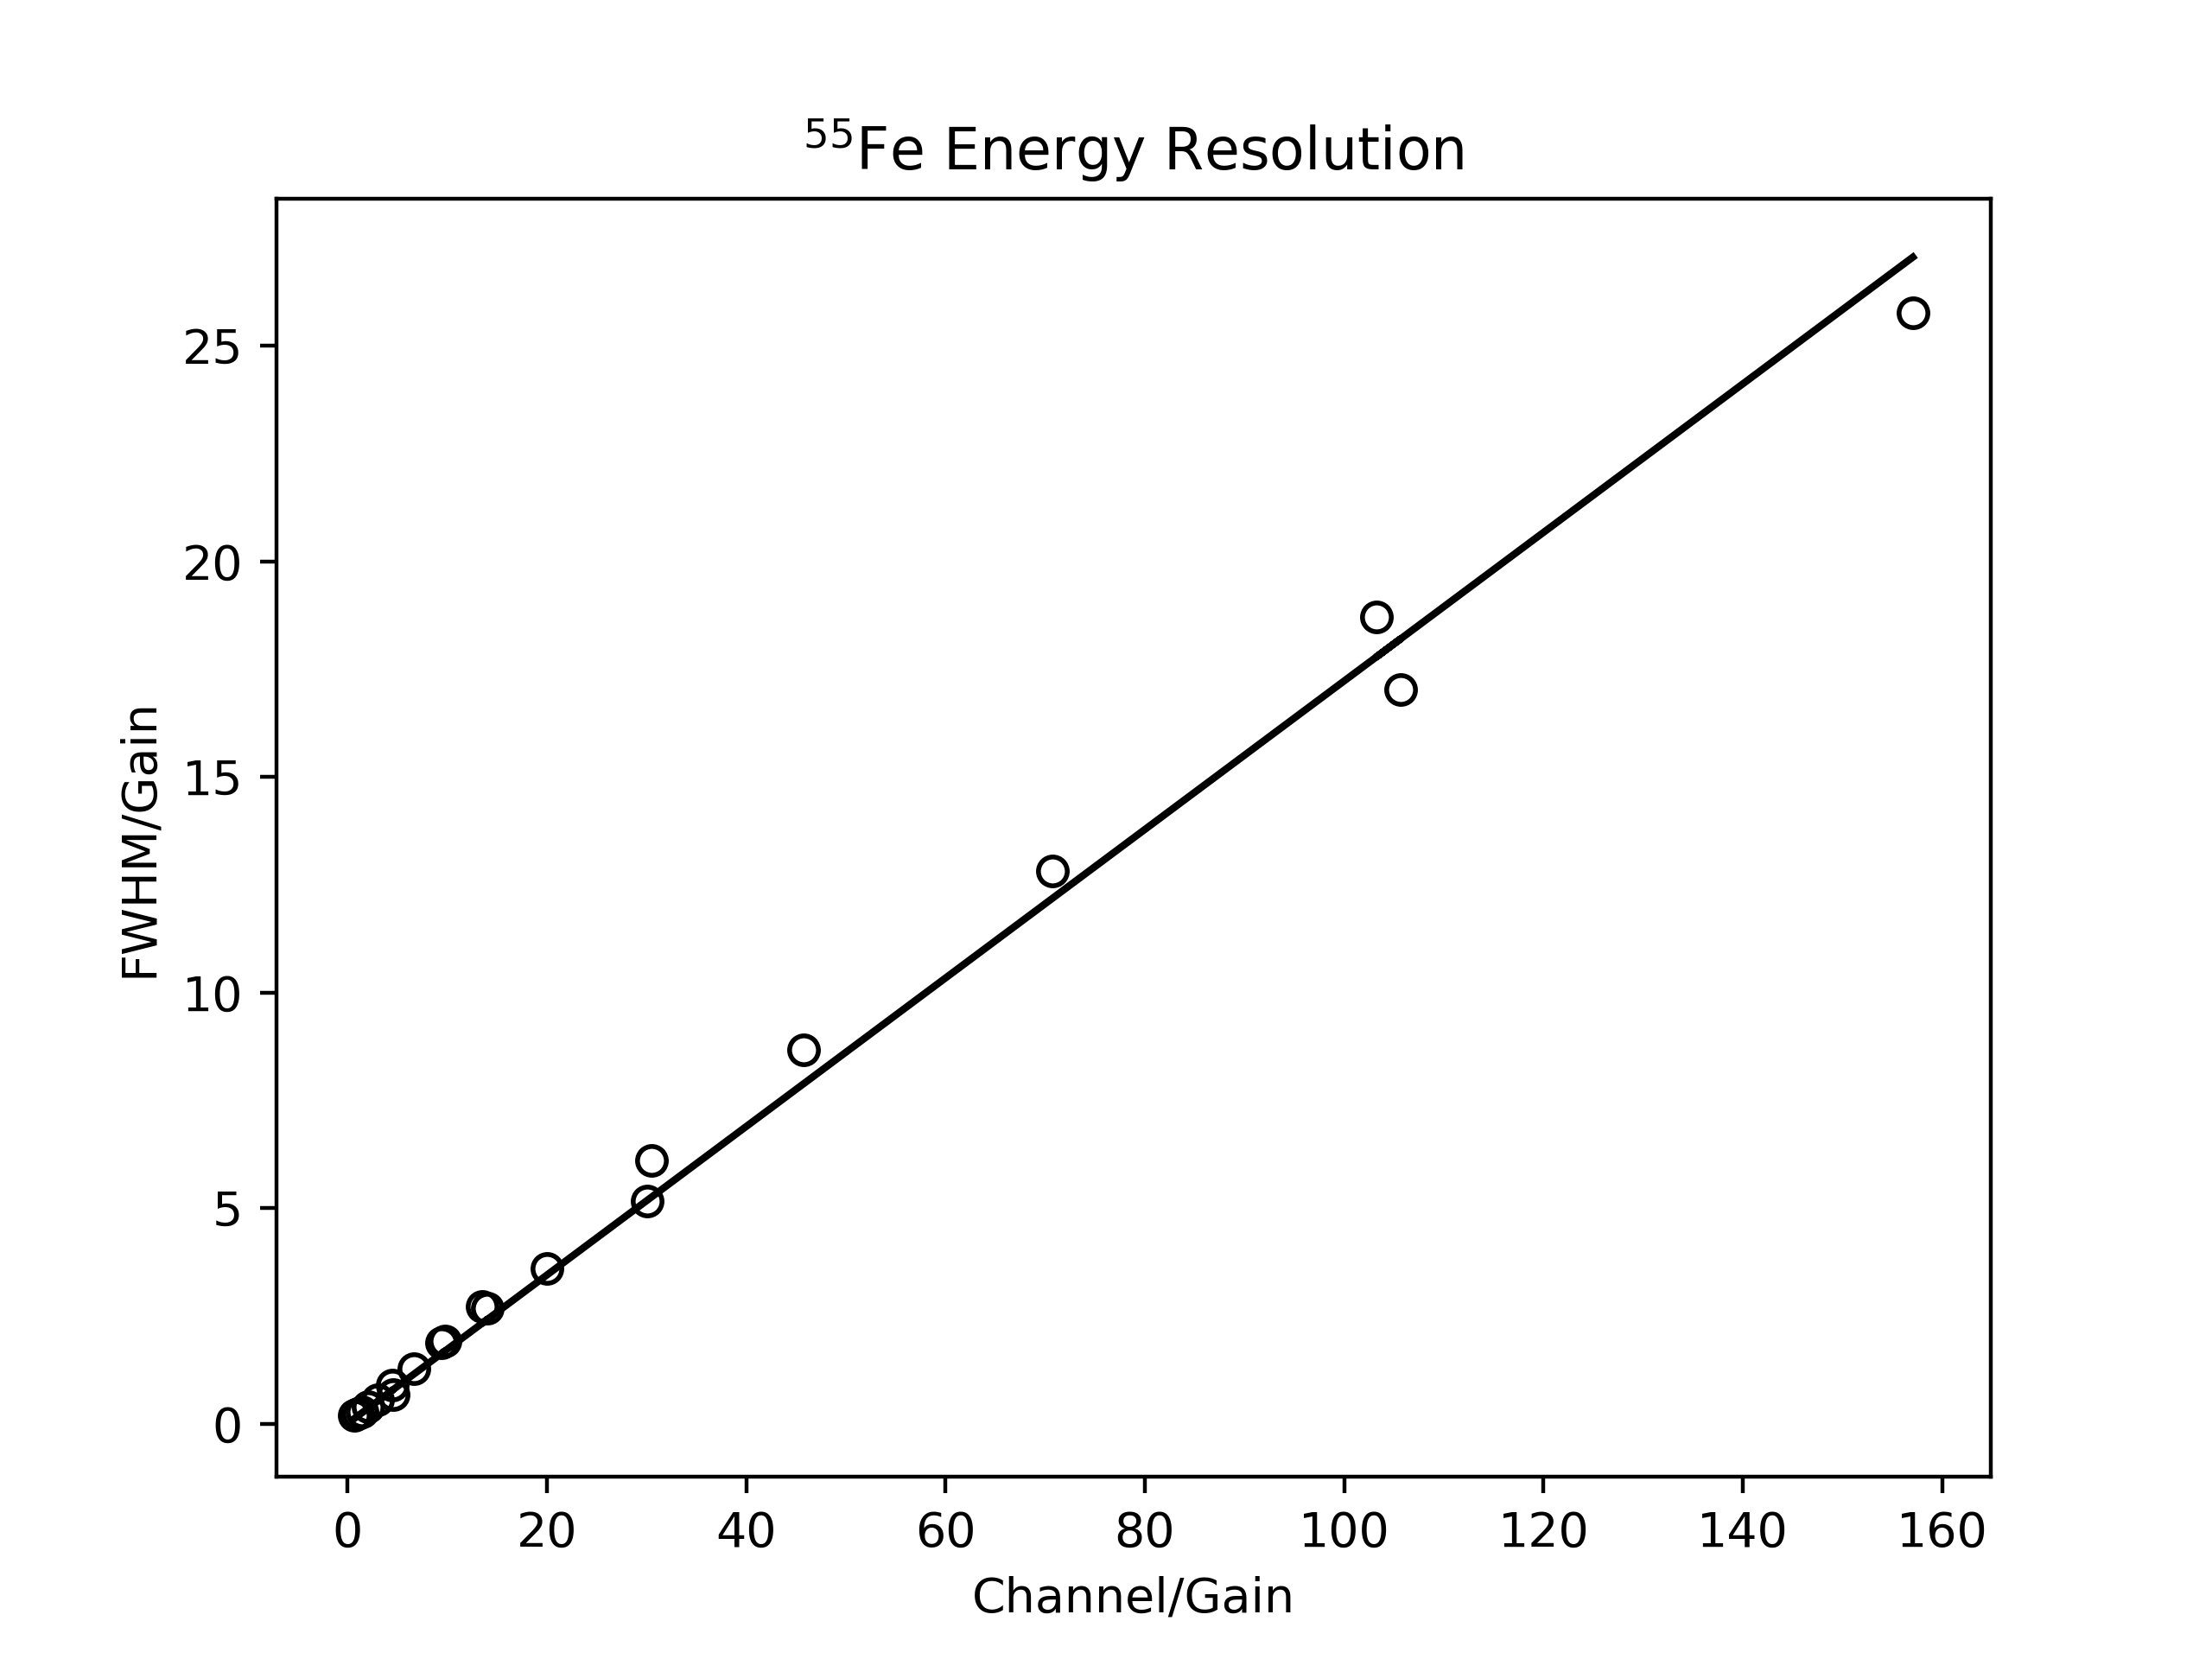
\includegraphics[width=12cm]{energyResolutionFe.png}
  \caption{Graph of gain corrected FWHM against centroid channel for \textsuperscript{55}Fe. The gradient of the trend line is E\textsubscript{res} = (17.2$\pm$0.5)\%.}
  \label{fig:energyResolutionFe}
\end{figure}

\begin{figure}[H]
  \centering
  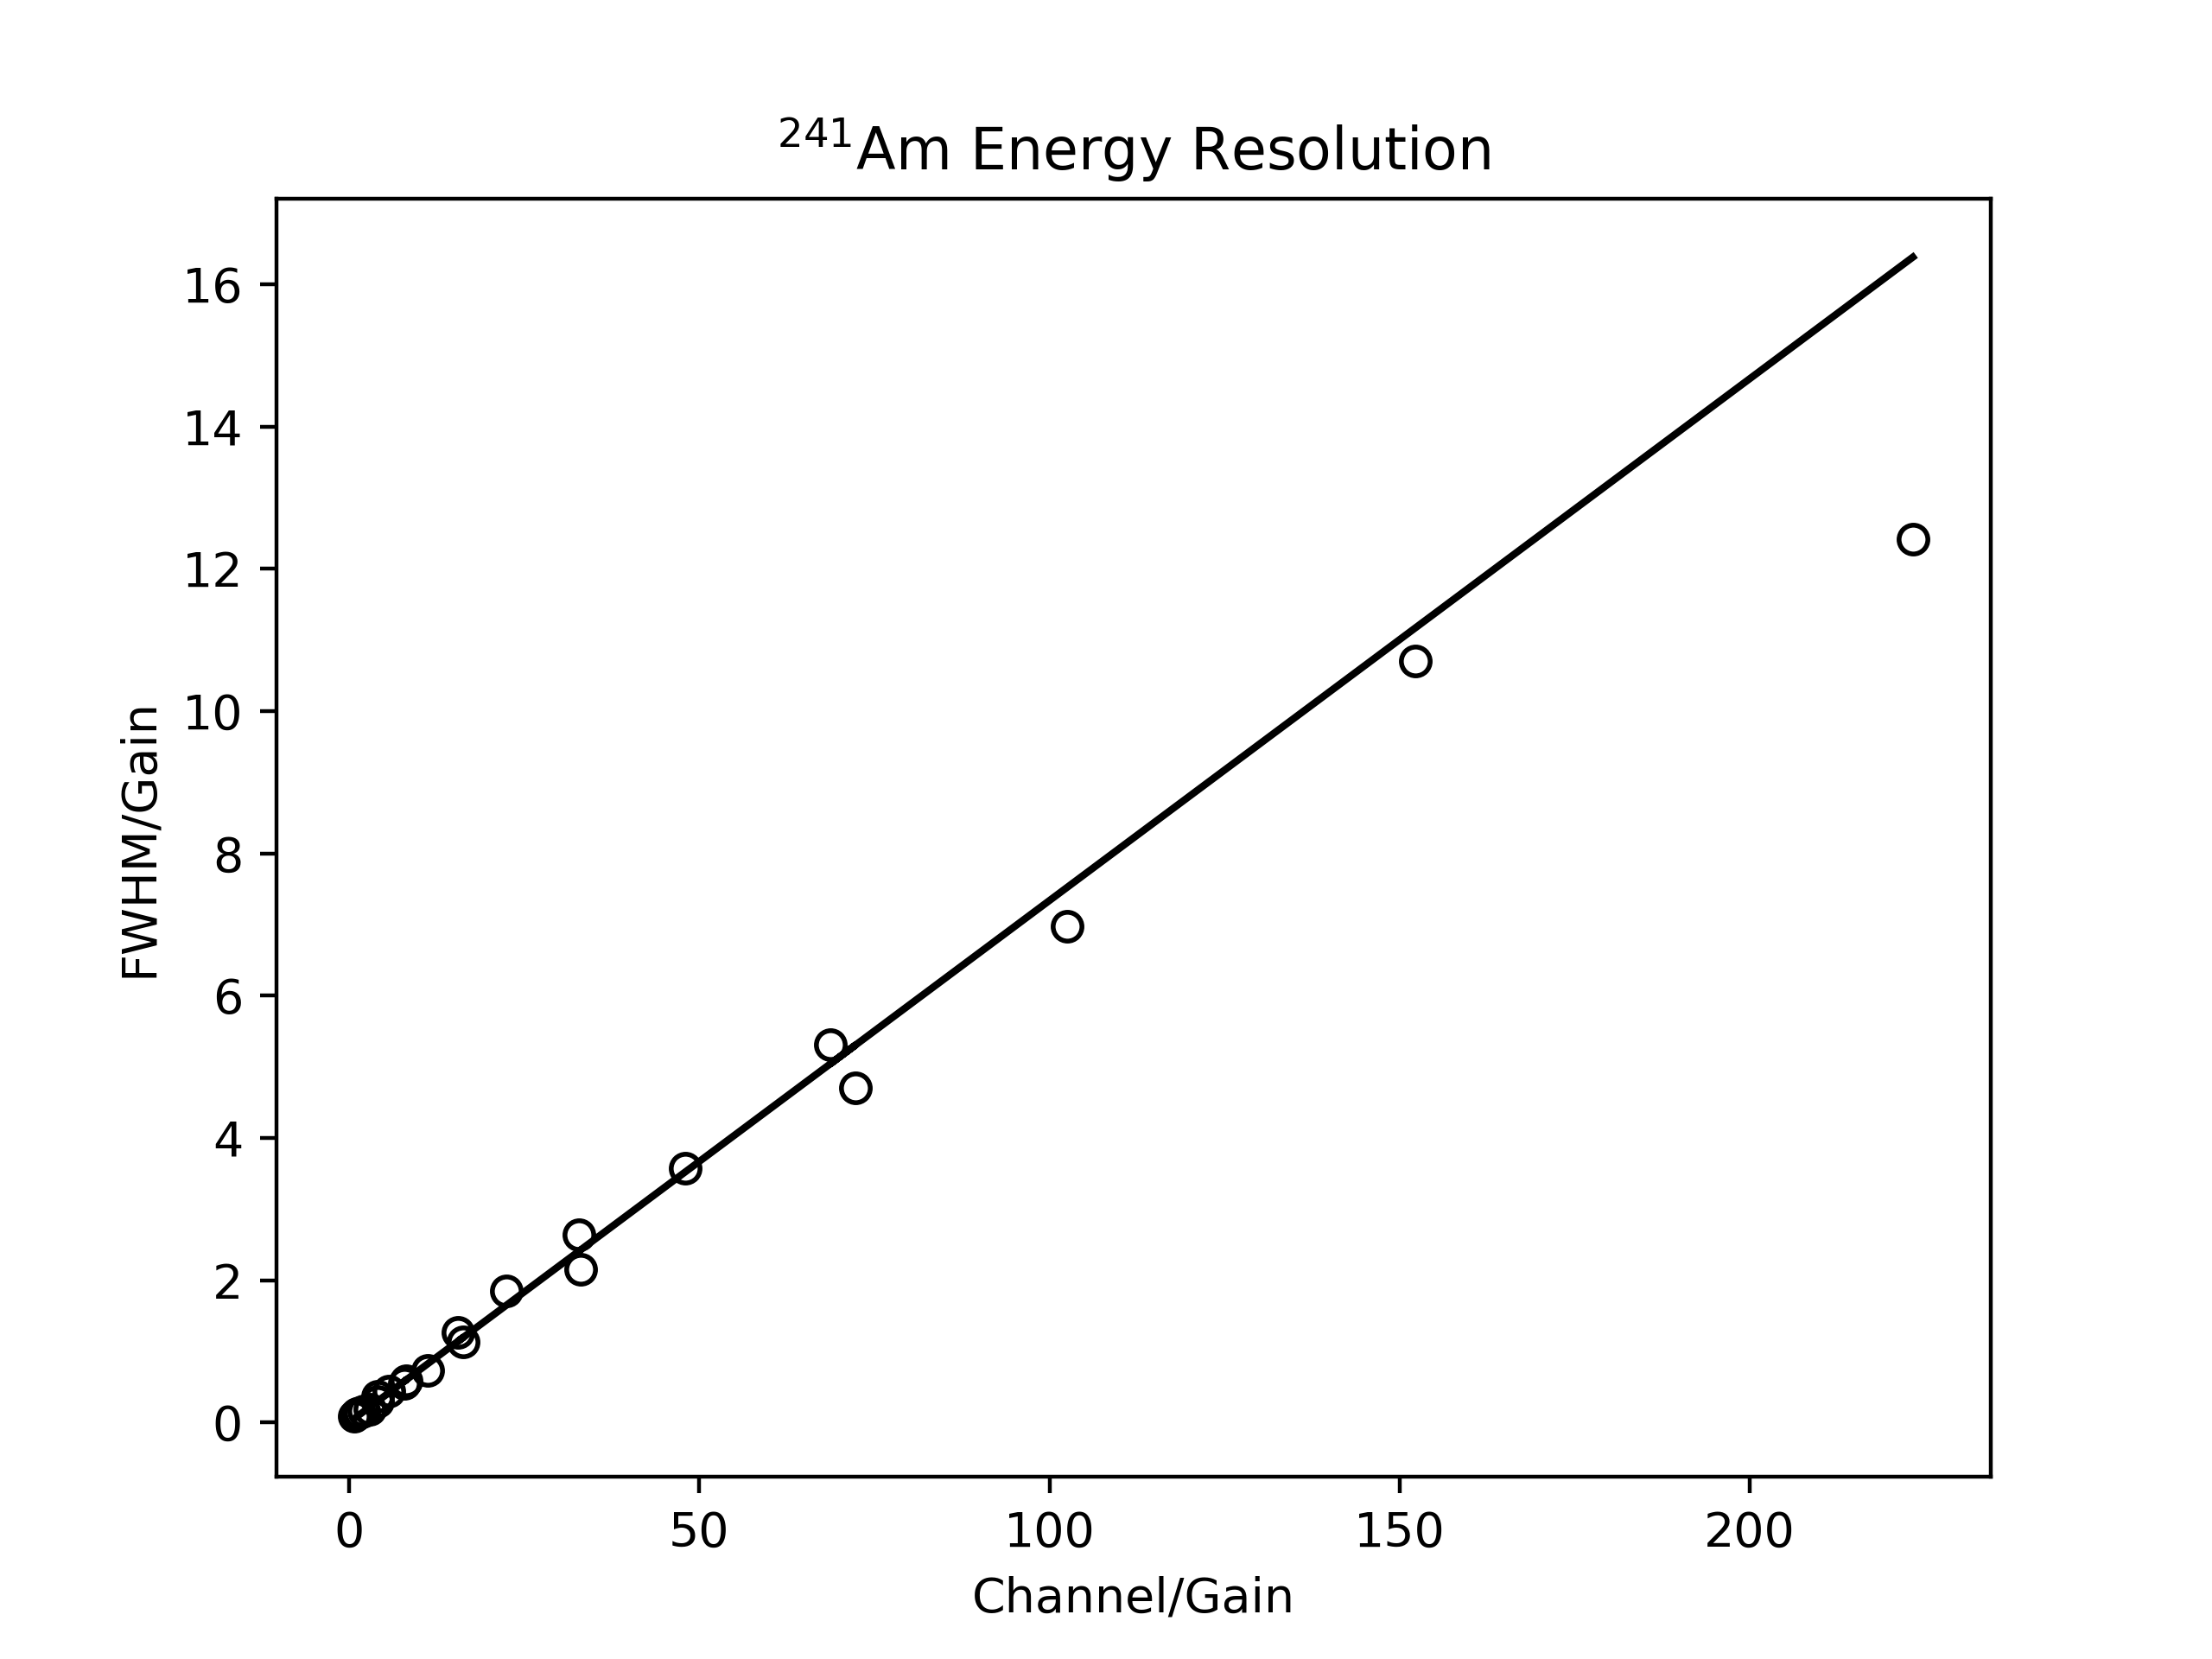
\includegraphics[width=12cm]{energyResolutionAm.png}
  \caption{Graph of gain corrected FWHM against centroid channel for \textsuperscript{241}Am. The gradient of the trend line is E\textsubscript{res} = (7.3$\pm$0.2)\%.}
  \label{fig:energyResolutionAm}
\end{figure}

\begin{figure}[H]
  \centering
  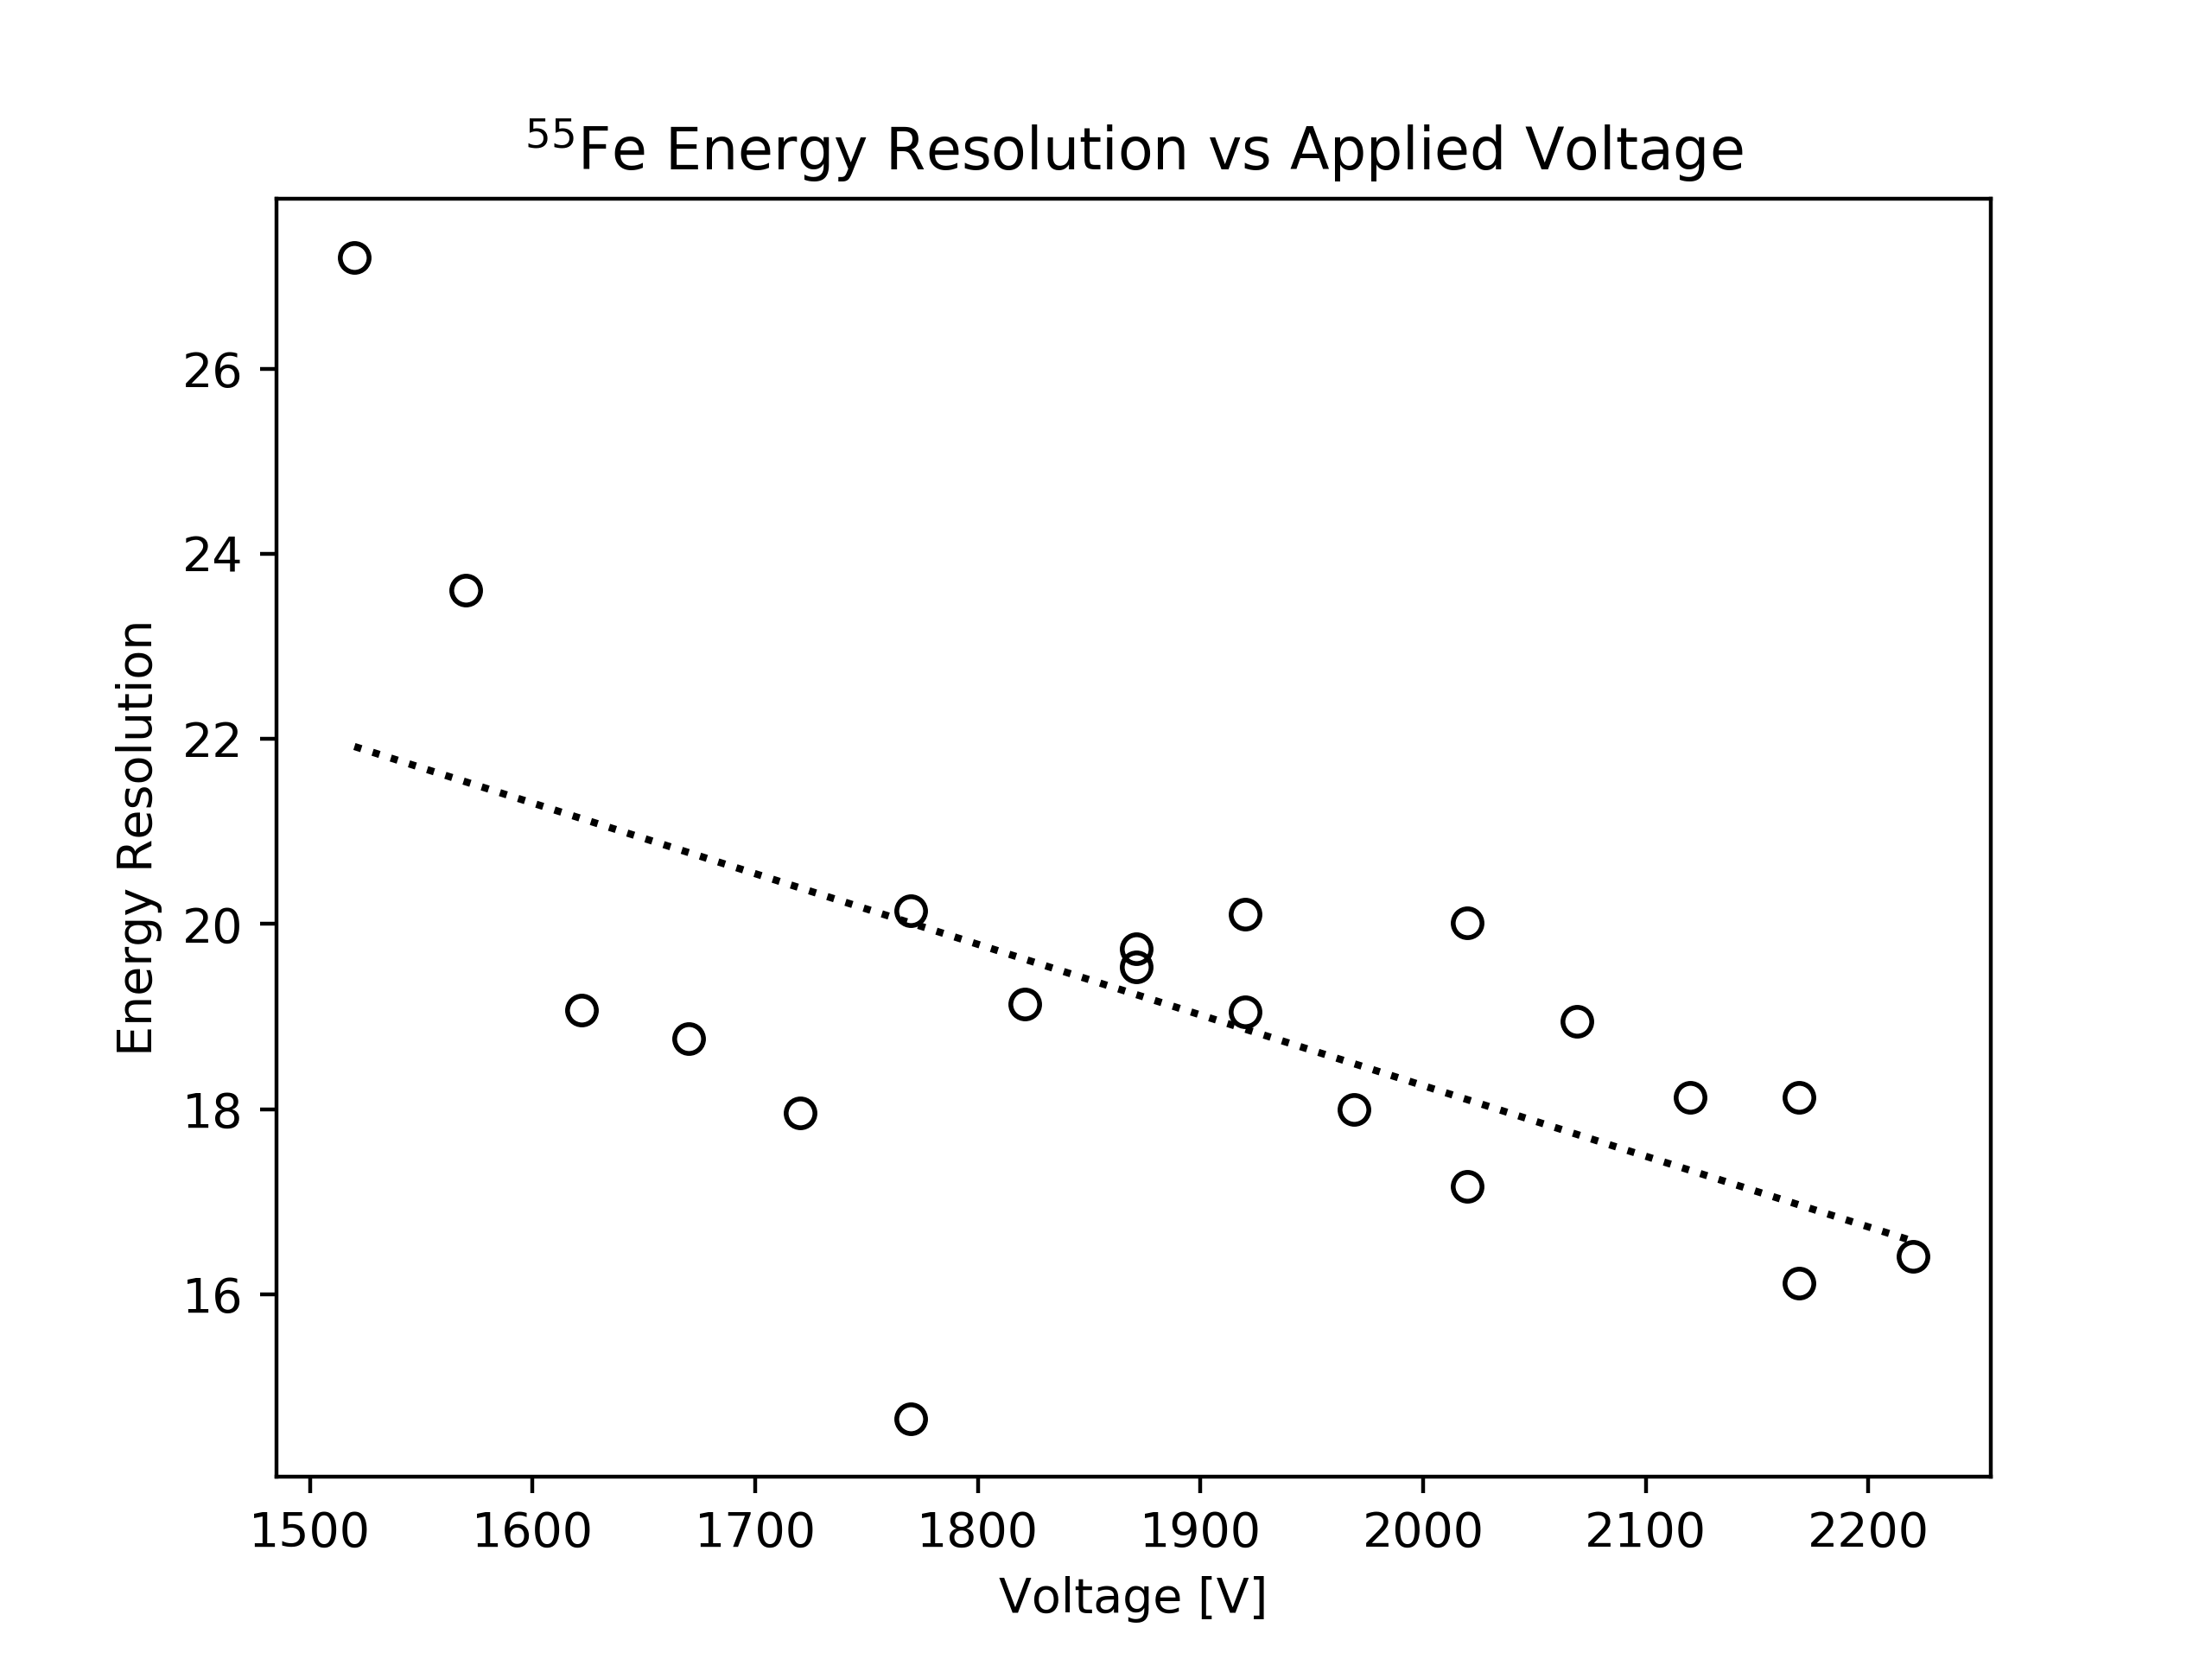
\includegraphics[width=12cm]{EResVsVFe.png}
  \caption{Graph of the energy resolution while measuring \textsuperscript{55}Fe, plotted against applied voltage.}
  \label{fig:EResVsVFe}
\end{figure}

\begin{figure}[H]
  \centering
  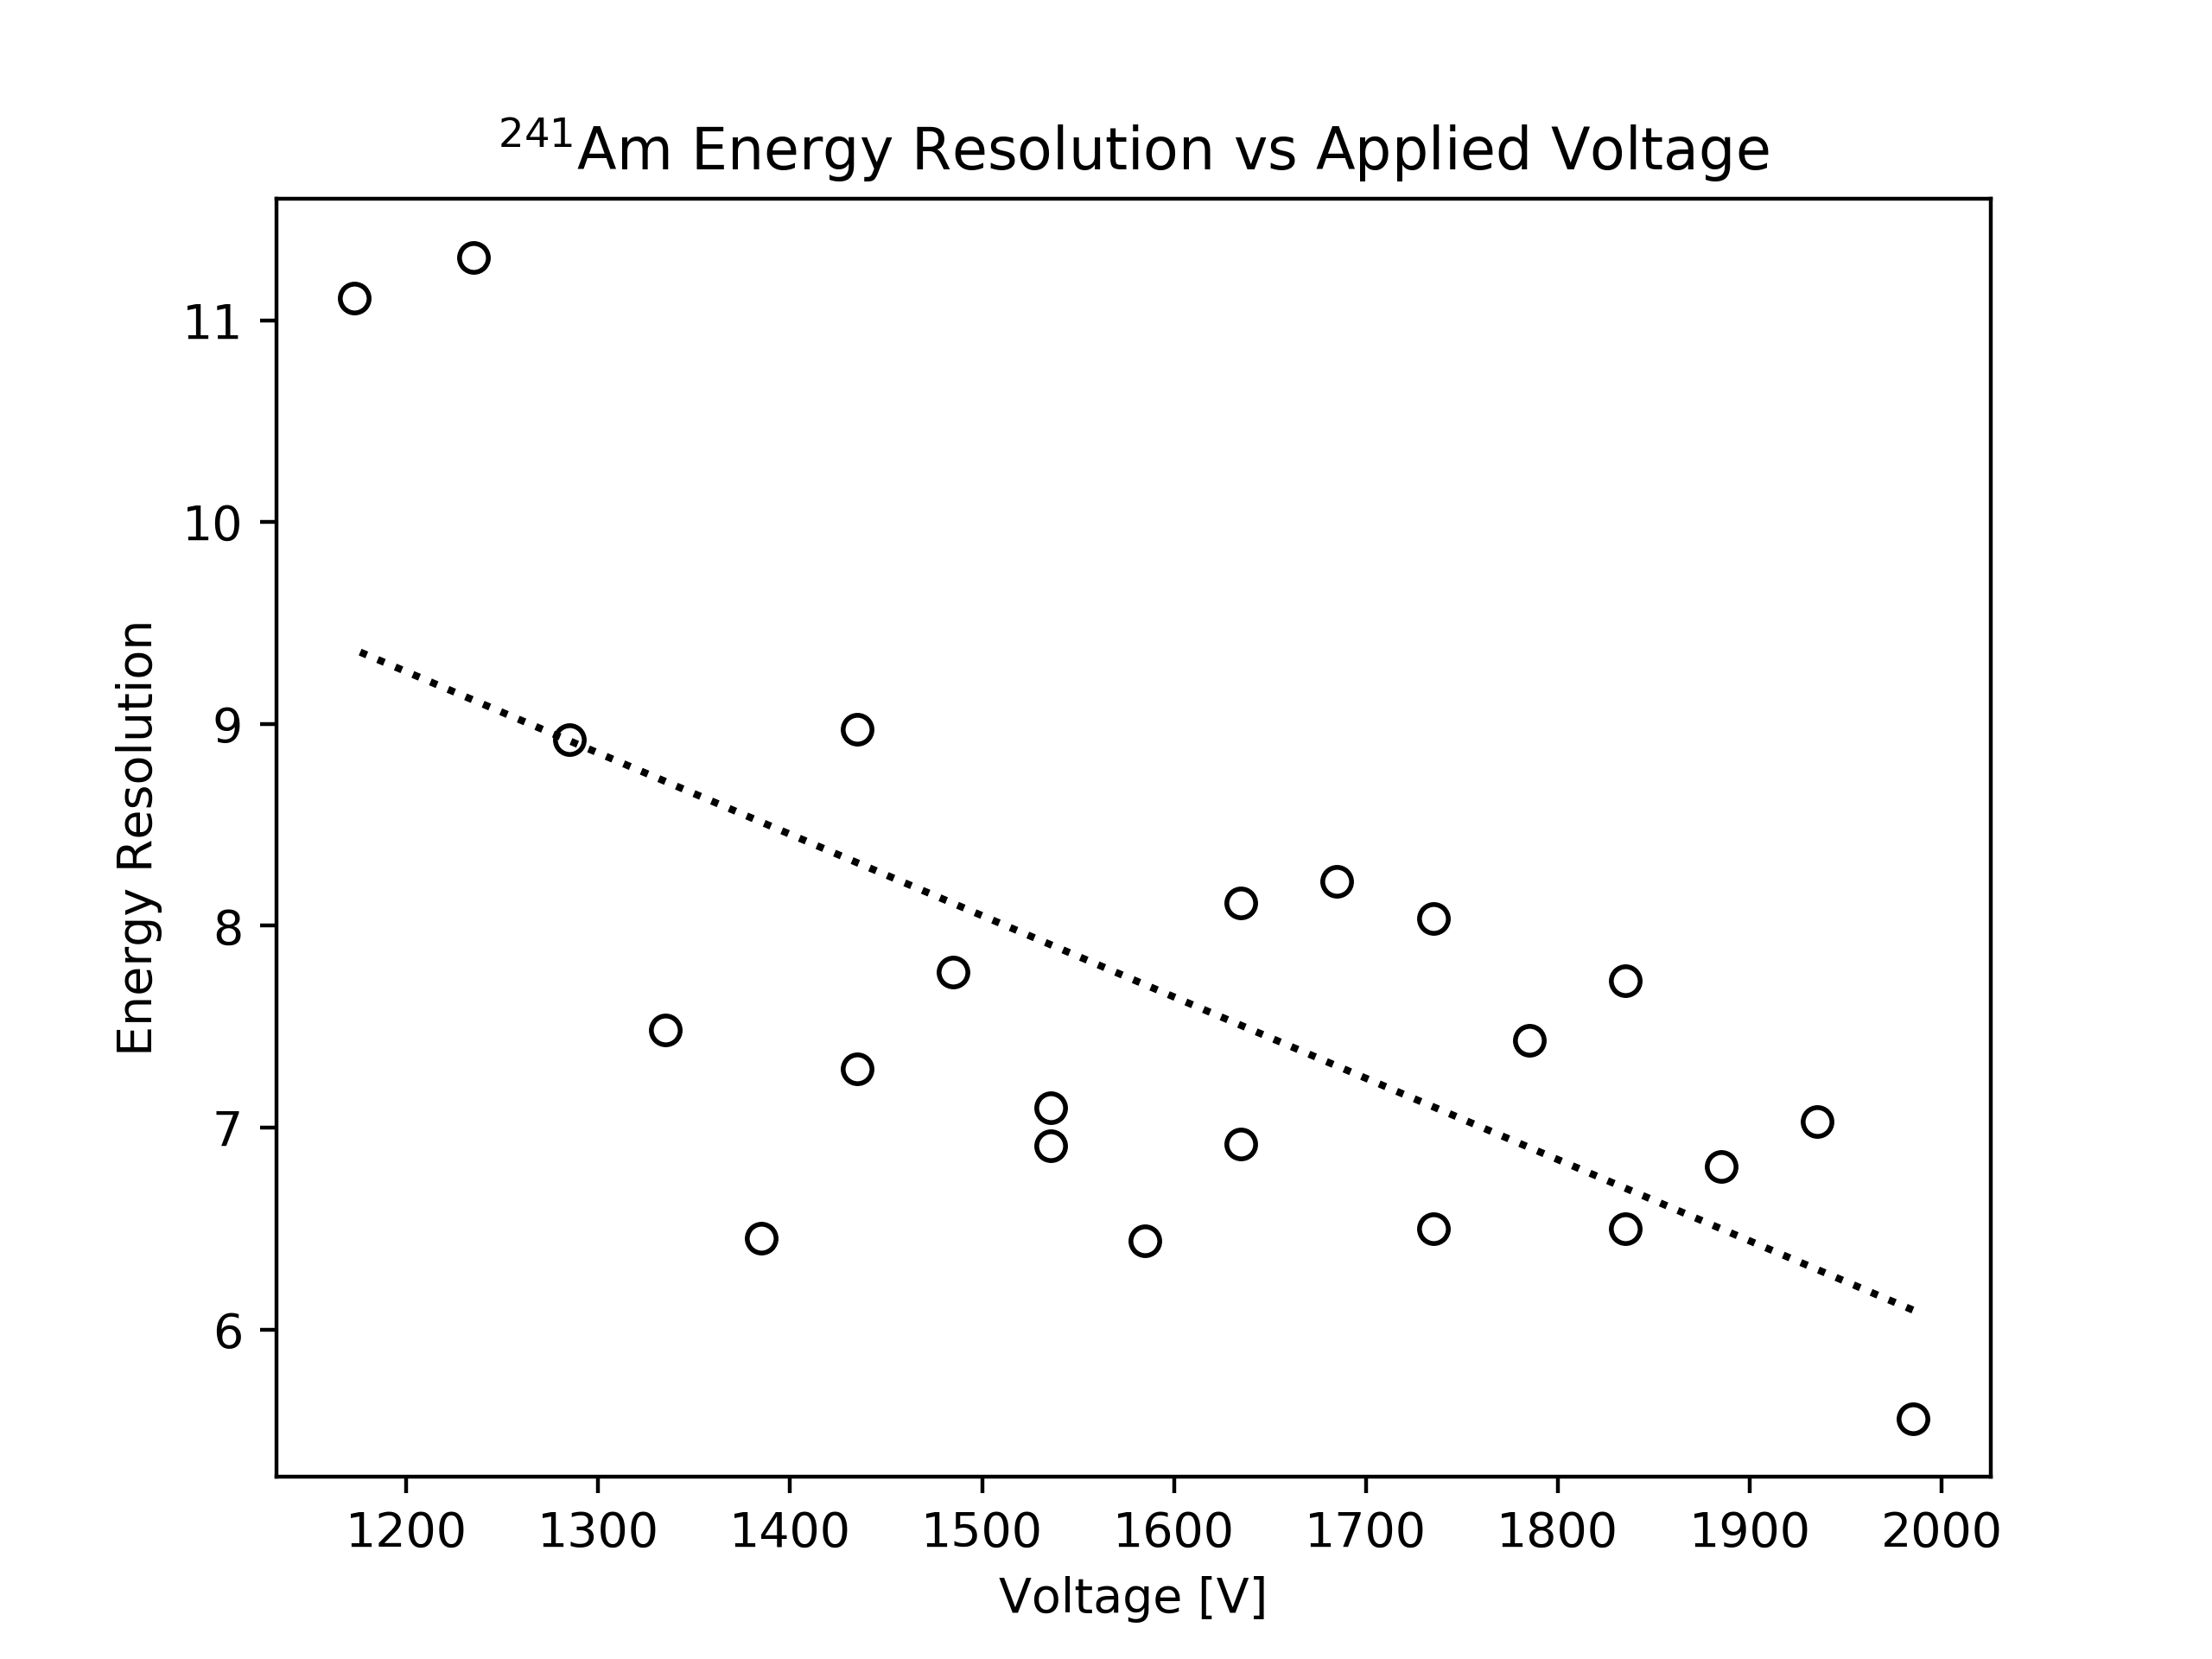
\includegraphics[width=12cm]{EResVsVAm.png}
  \caption{Graph of the energy resolution while measuring \textsuperscript{241}Am, plotted against applied voltage.}
  \label{fig:EResVsVAm}
\end{figure}

\subsection{Spectra}

\begin{figure}[H]
  \centering
  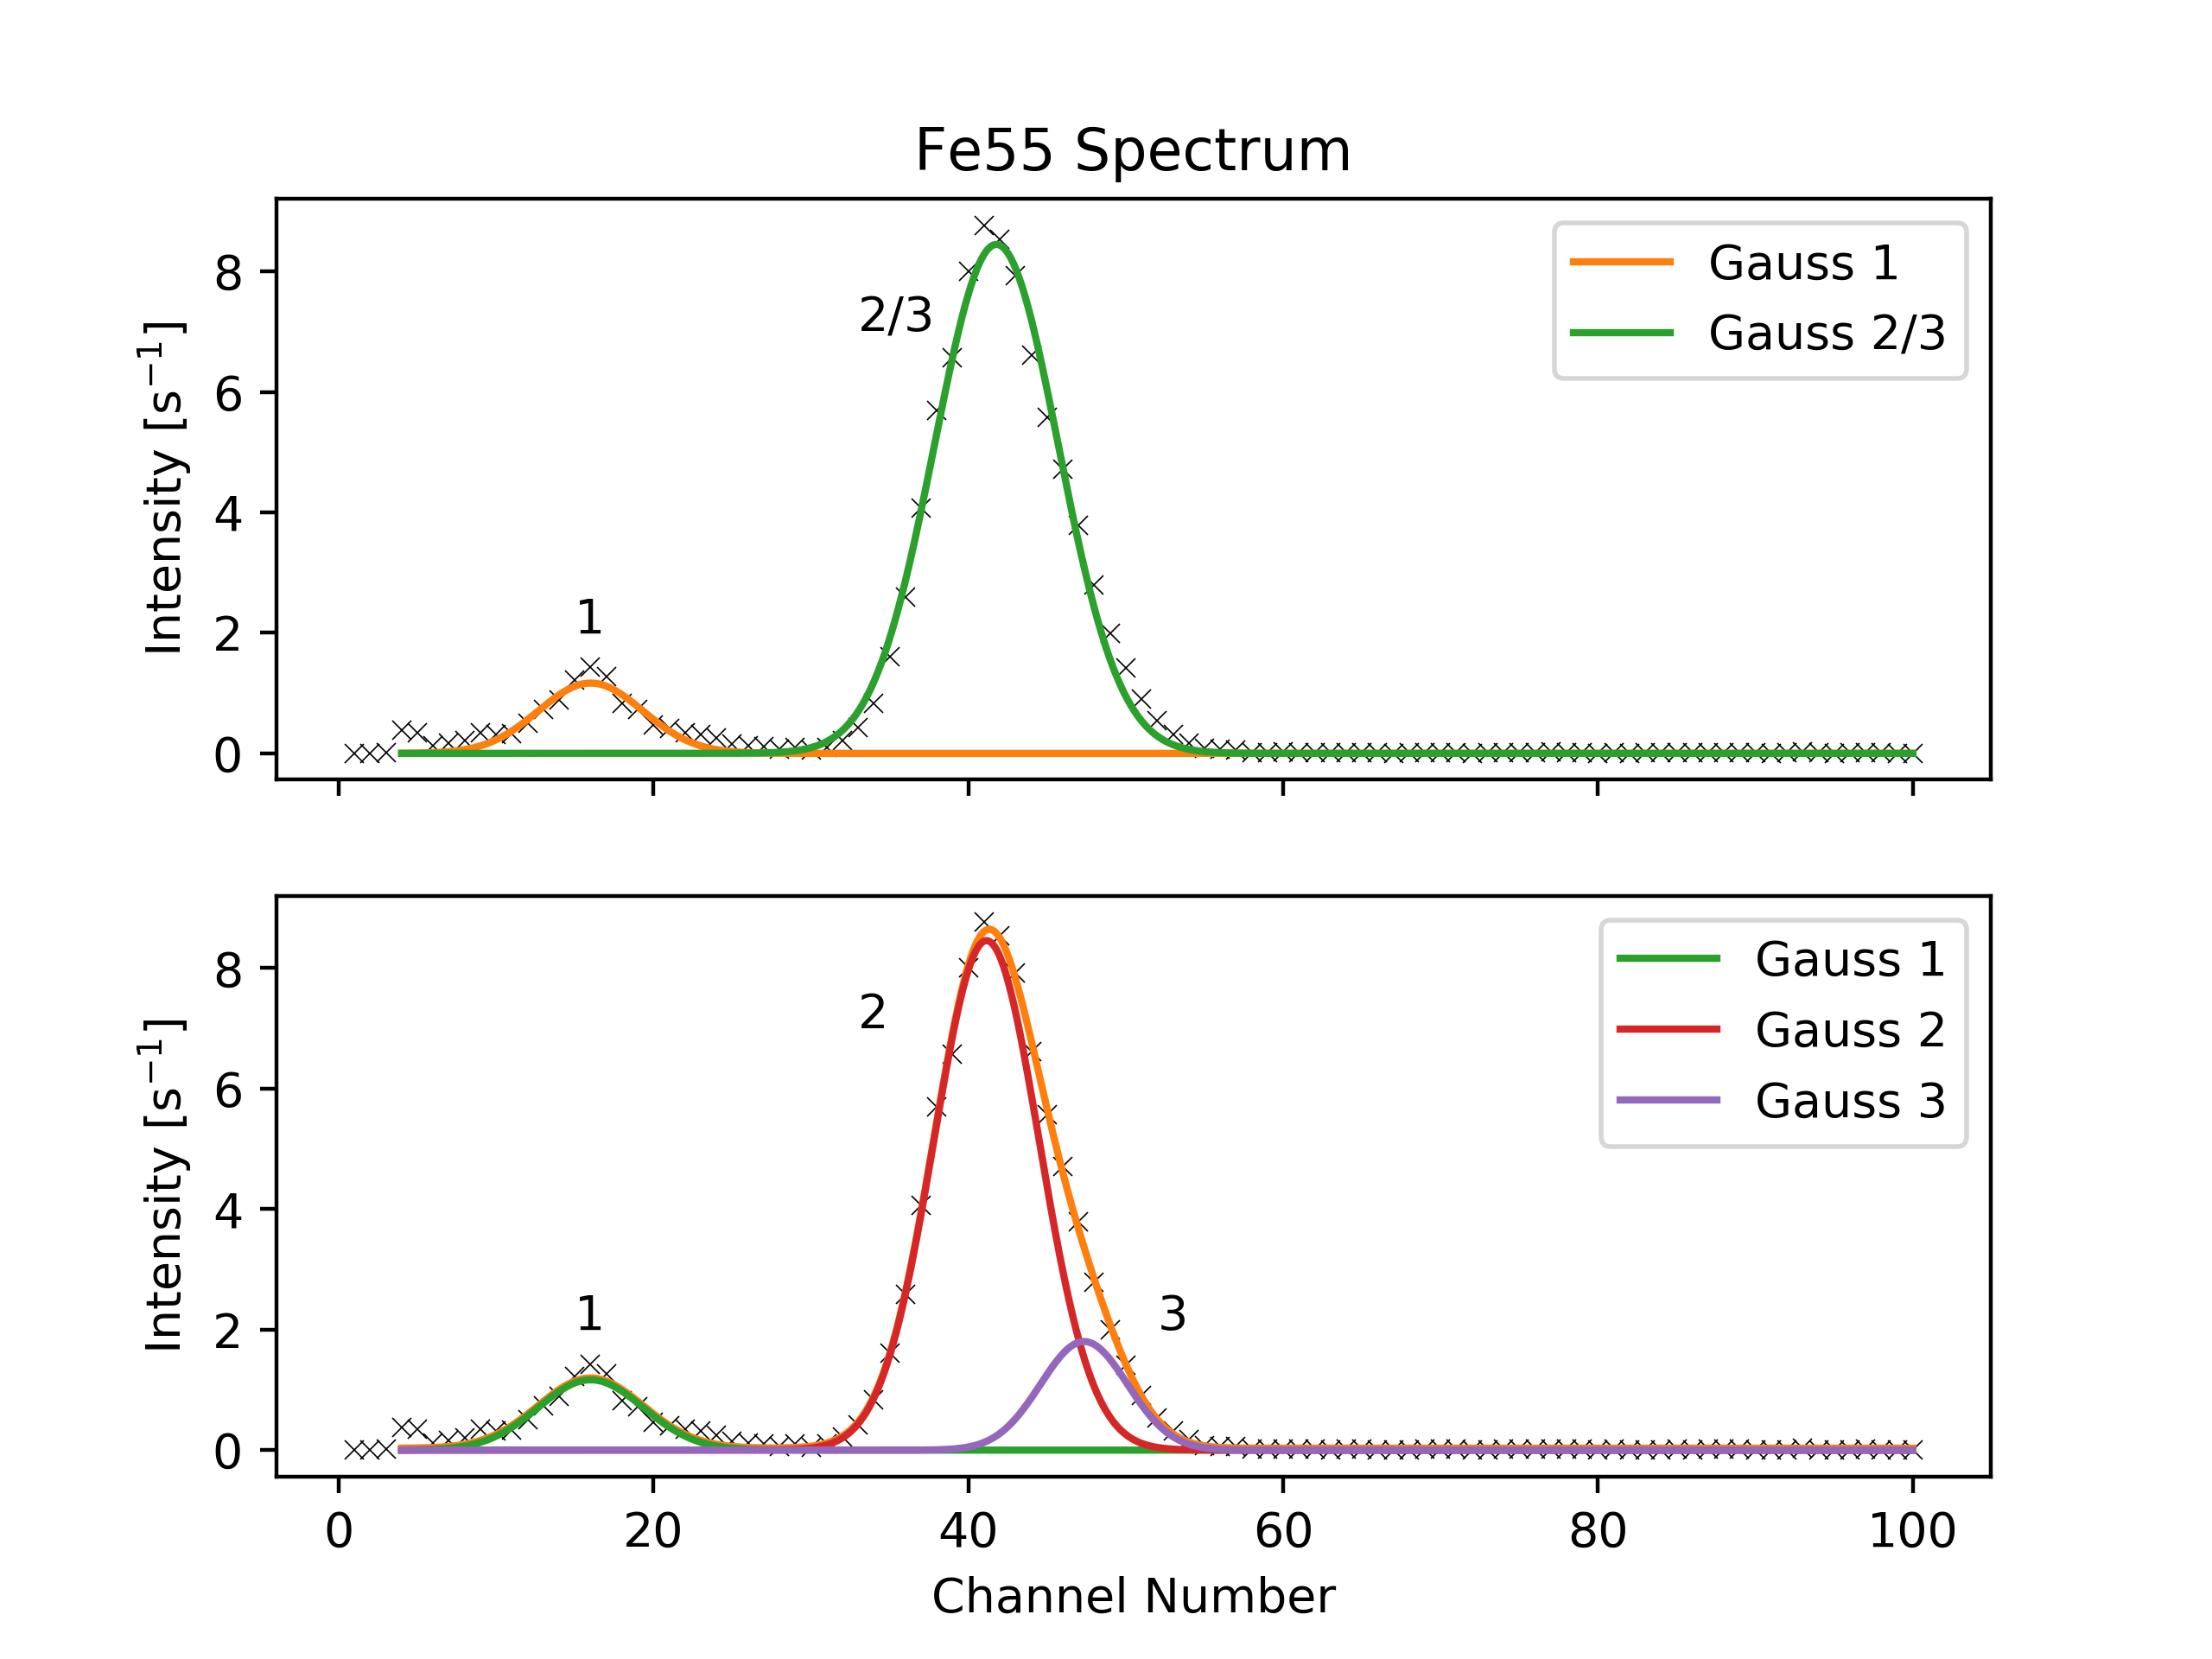
\includegraphics[width=9.93cm]{Fe55_spectrum.png}
  \caption{The spectrum of \textsuperscript{55}Fe from channels 0 to 100 because above 100 there were no spectral features. The top graph models the main photopeak as a single Gaussian curve, the bottom models it as two. The background in both cases was found to be almost negligible: (0.4$\pm$0.2) top; (0.3$\pm$0.1) bottom. The peak centres and FHWM are compiled in Table \ref{tbl:energyCalibration}.}
  \label{fig:Fe55spec}
\end{figure}

\begin{figure}[H]
  \centering
  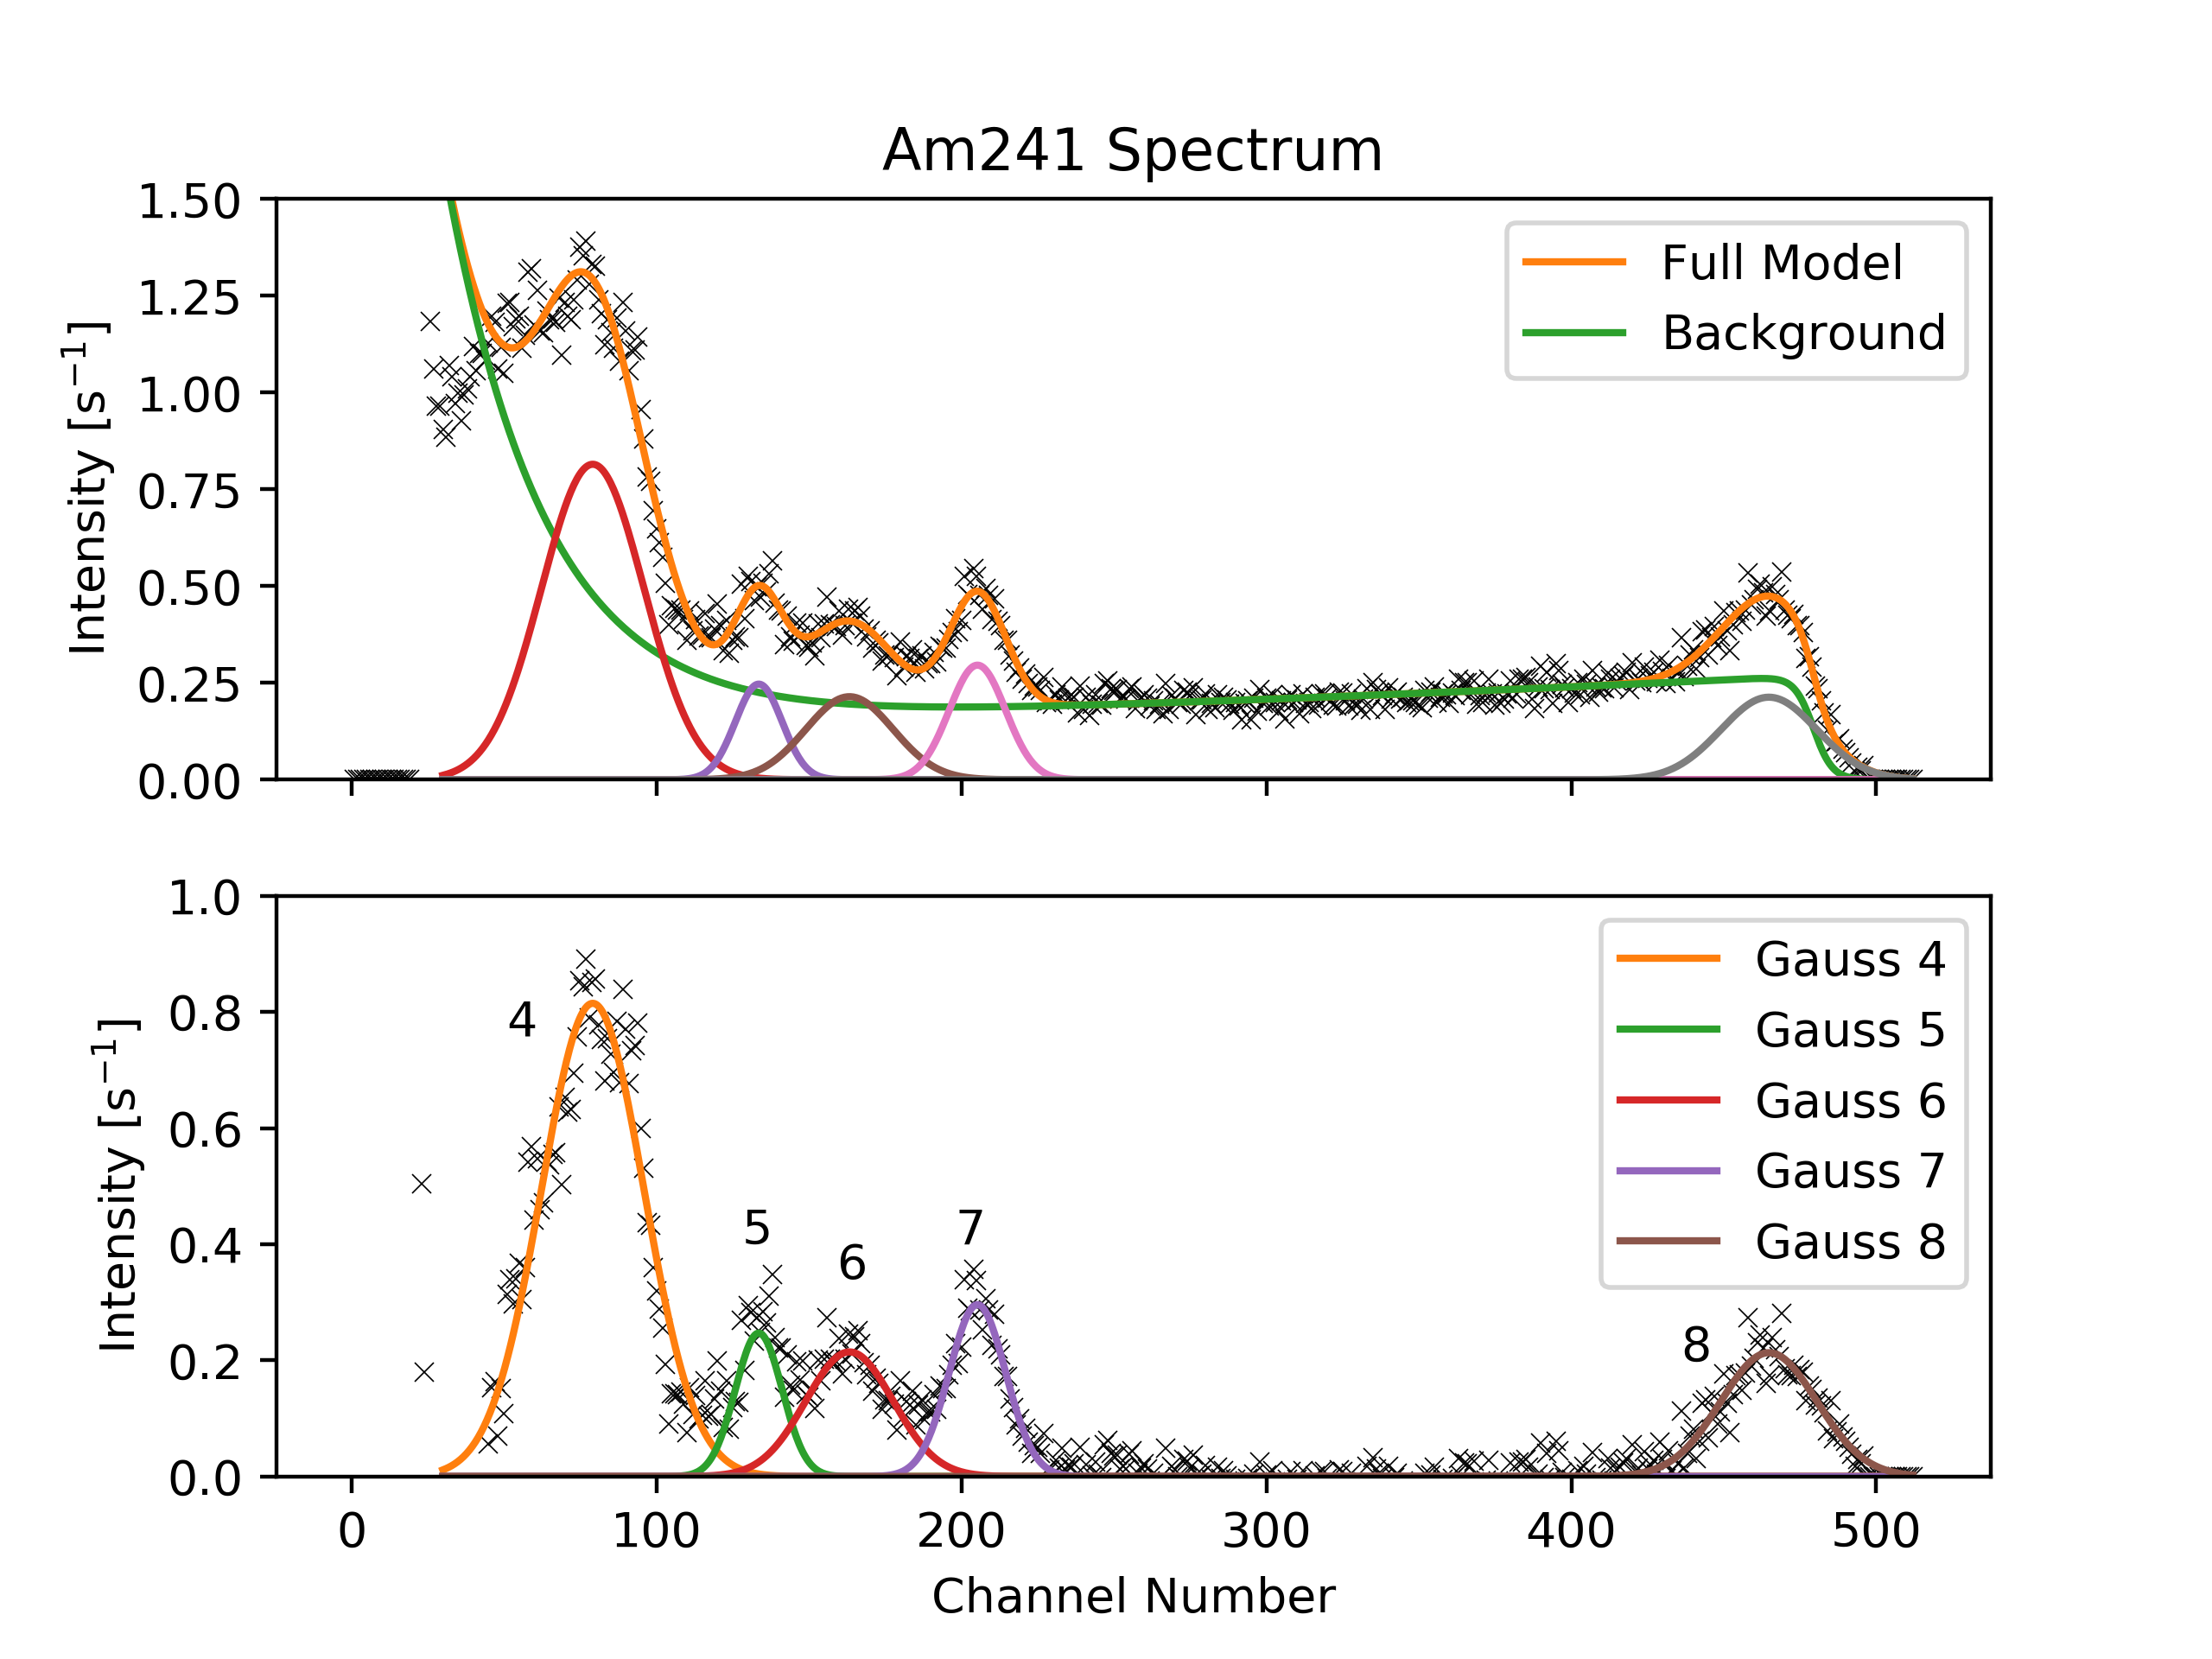
\includegraphics[width=9.93cm]{Am241_spectrum.png}
  \caption{The top graph shows the full spectrum of \textsuperscript{241}Am and the fitted model. The bottom graph shows the spectrum minus the background, leaving just the peaks. The parameters for the background were found to be: a$_{1}$ = (3.7$\pm$0.9), b$_{1}$ = (-0.030$\pm$0.007), a$_{2}$ = (0.13$\pm$0.01), b$_{2}$ = (0.0014$\pm$0.0003), c = (479$\pm$1), d = (3.1$\pm$0.8). The peak centres and FHWM are compiled in Table \ref{tbl:energyCalibration}.}
  \label{fig:Am241spec}
\end{figure}

\subsection{Energy Calibration}

\begin{table}[H]
    \begin{tabular}{llll}
    \hline \hline
    Peak & Channel  & Energy [keV] & FWHM [keV]  \\ \hline
    1    & 16.0$\pm$1    & 3.20 (Calib.)          & 0.97$\pm$0.02   \\
    2    & 41.2$\pm$0.1  & 5.89 (Calib.)        & 0.975$\pm$0.009 \\
    3    & 47.3$\pm$0.5  & 6.49 (Calib.)        & 0.80$\pm$0.03   \\
    4    & 79.1$\pm$0.4  & 10.78$\pm$0.05   & 4.9$\pm$0.2     \\
    5    & 133.6$\pm$0.9 & 17.5$\pm$0.1     & 2.2$\pm$0.1     \\
    6    & 163$\pm$1     & 21.15$\pm$0.04   & 4.2$\pm$0.2     \\
    7    & 205.3$\pm$0.6 & 26.37$\pm$0.09      & 2.69$\pm$0.08   \\
    8    & 465$\pm$1    & 59.54 (Calib.)       & 4.6$\pm$0.2     \\ \hline \hline
    \end{tabular}
    \label{tbl:energyCalibration}
    \caption{Peak centres as found by fitting models to the spectra with their respective energies. Those used for calibration are denoted with (Calib.) and have no uncertainty as they are book values.}
\end{table}

\begin{figure}[H]
  \centering
  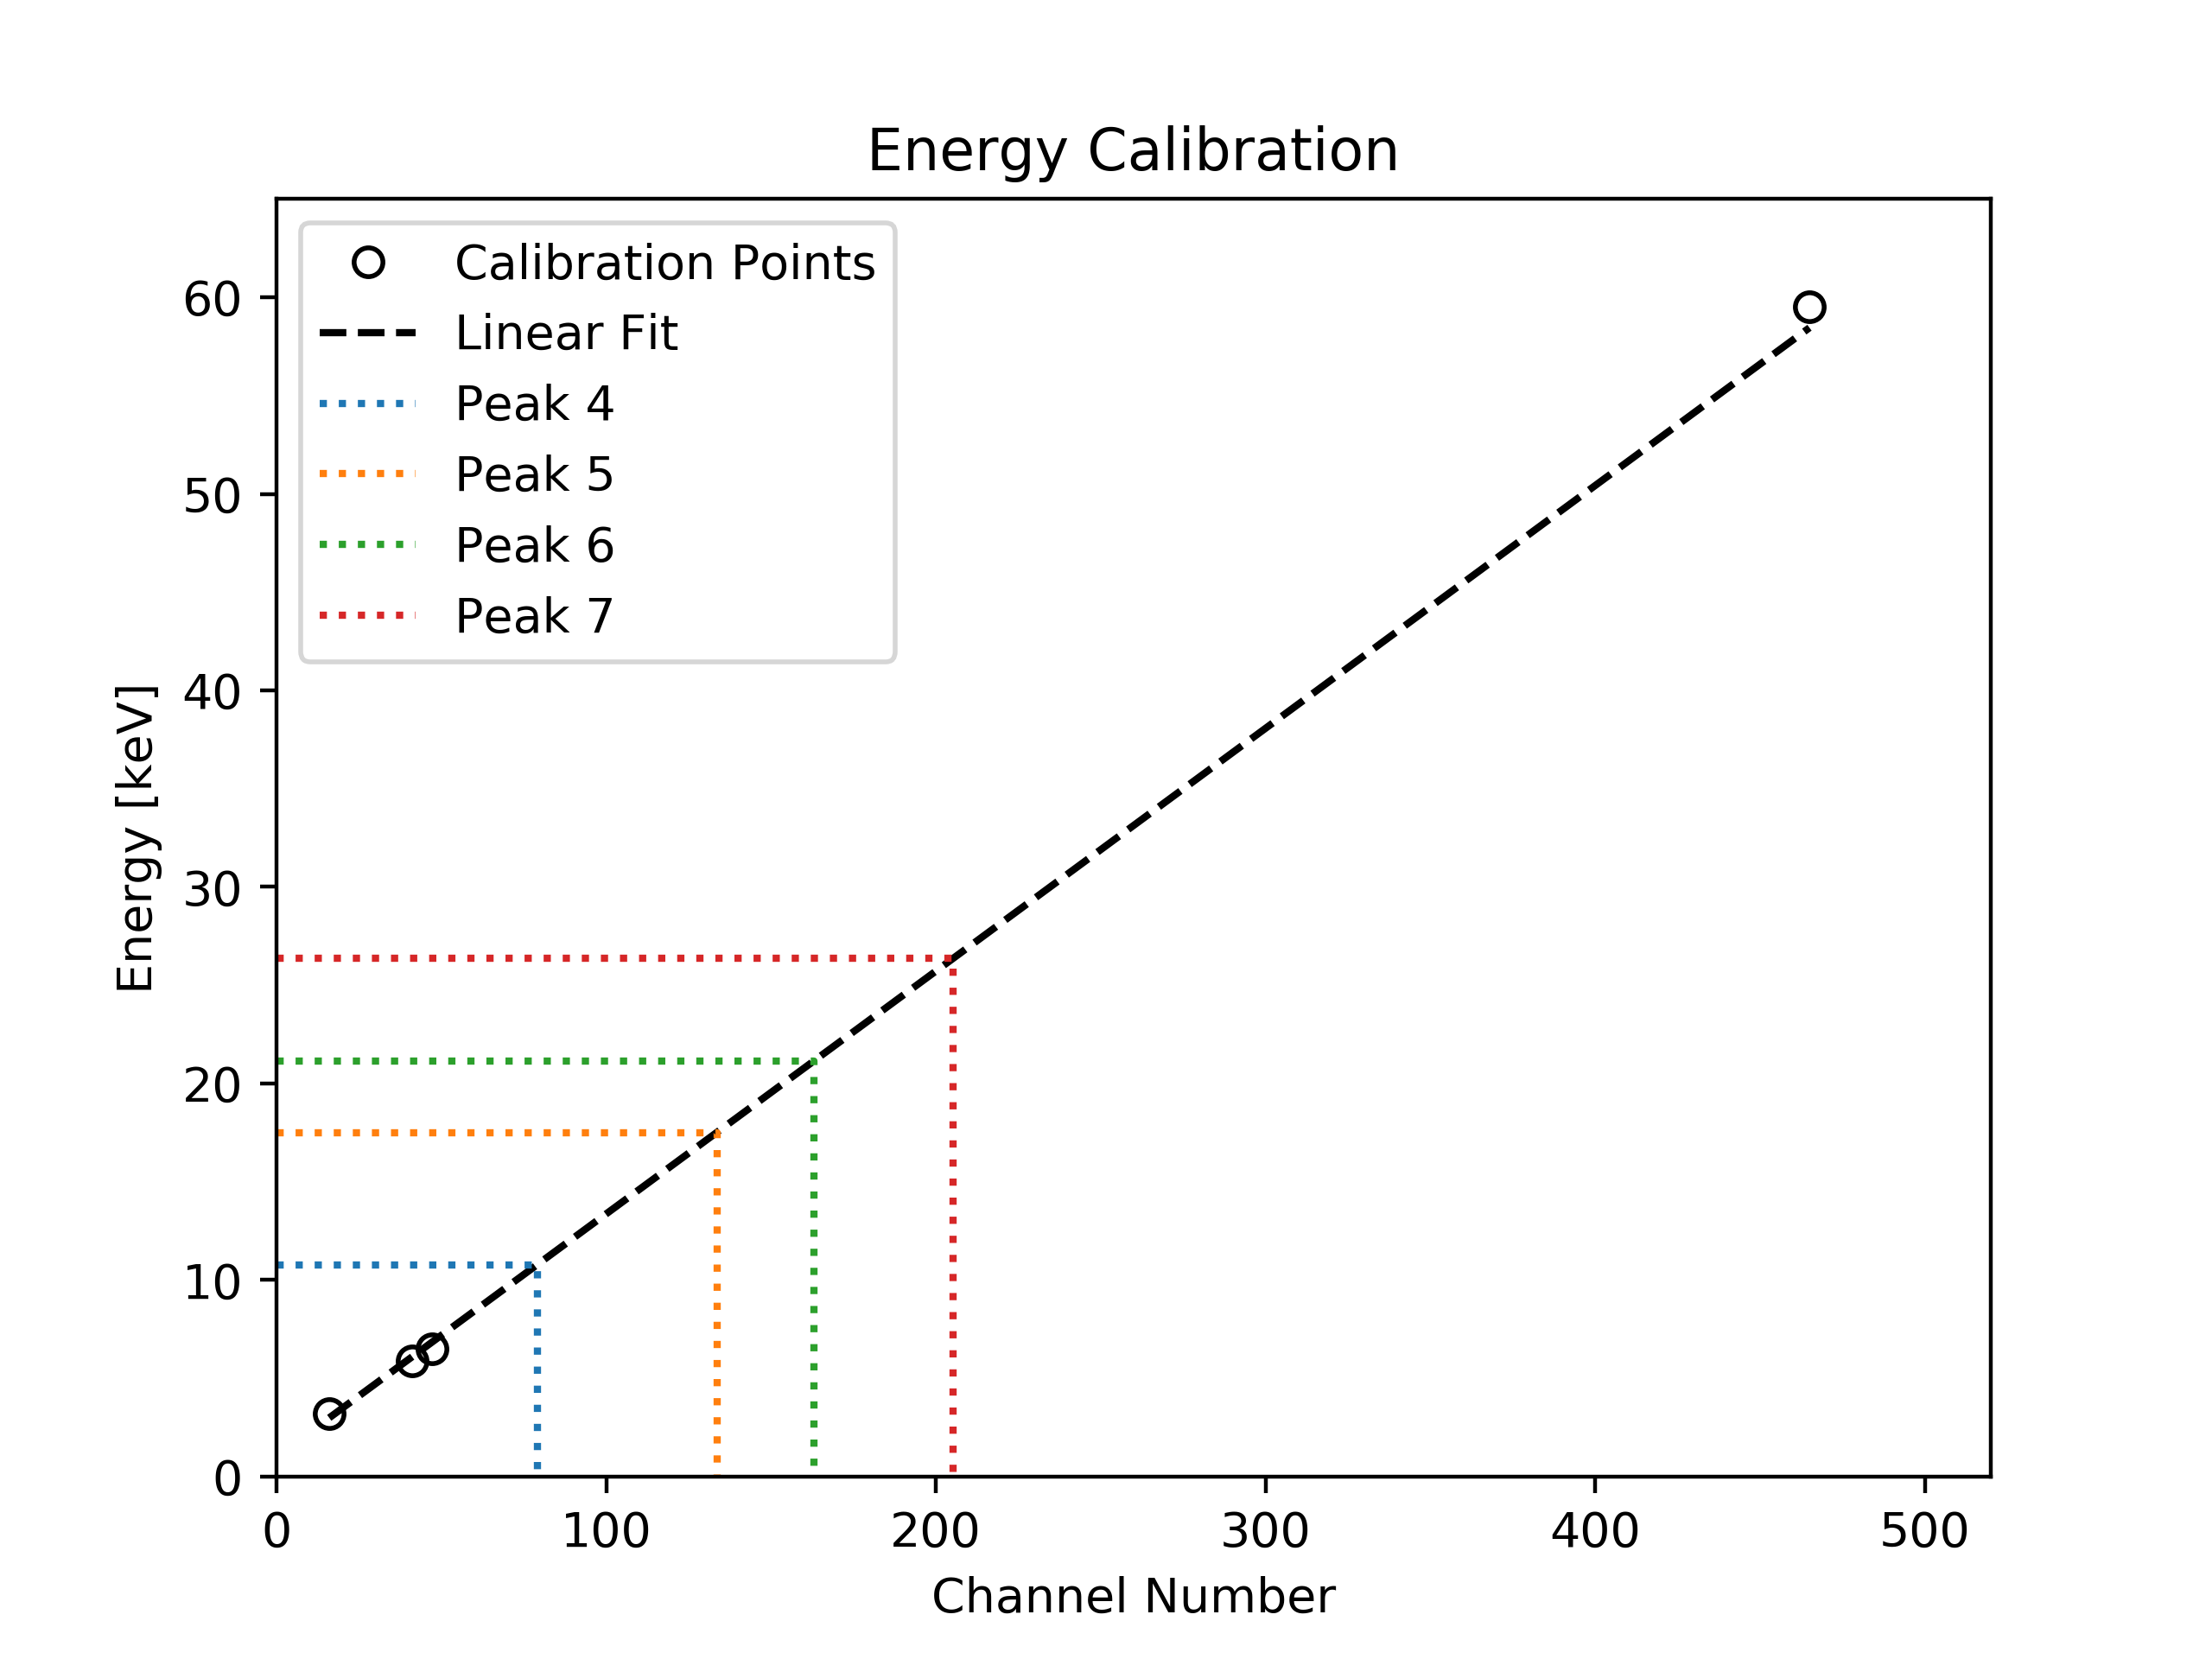
\includegraphics[width=\linewidth]{energyCalibration.png}
  \caption{Plot of channel centre against energy. The fitted linear model gave the conversion equation between particle energy and channel number to be: $E = (0.1235\pm0.0003)Ch + (1.01\pm0.01)$}
  \label{fig:energyCalibration}
\end{figure}

\section{Preamplifier}

\begin{figure}[H]
  \centering
  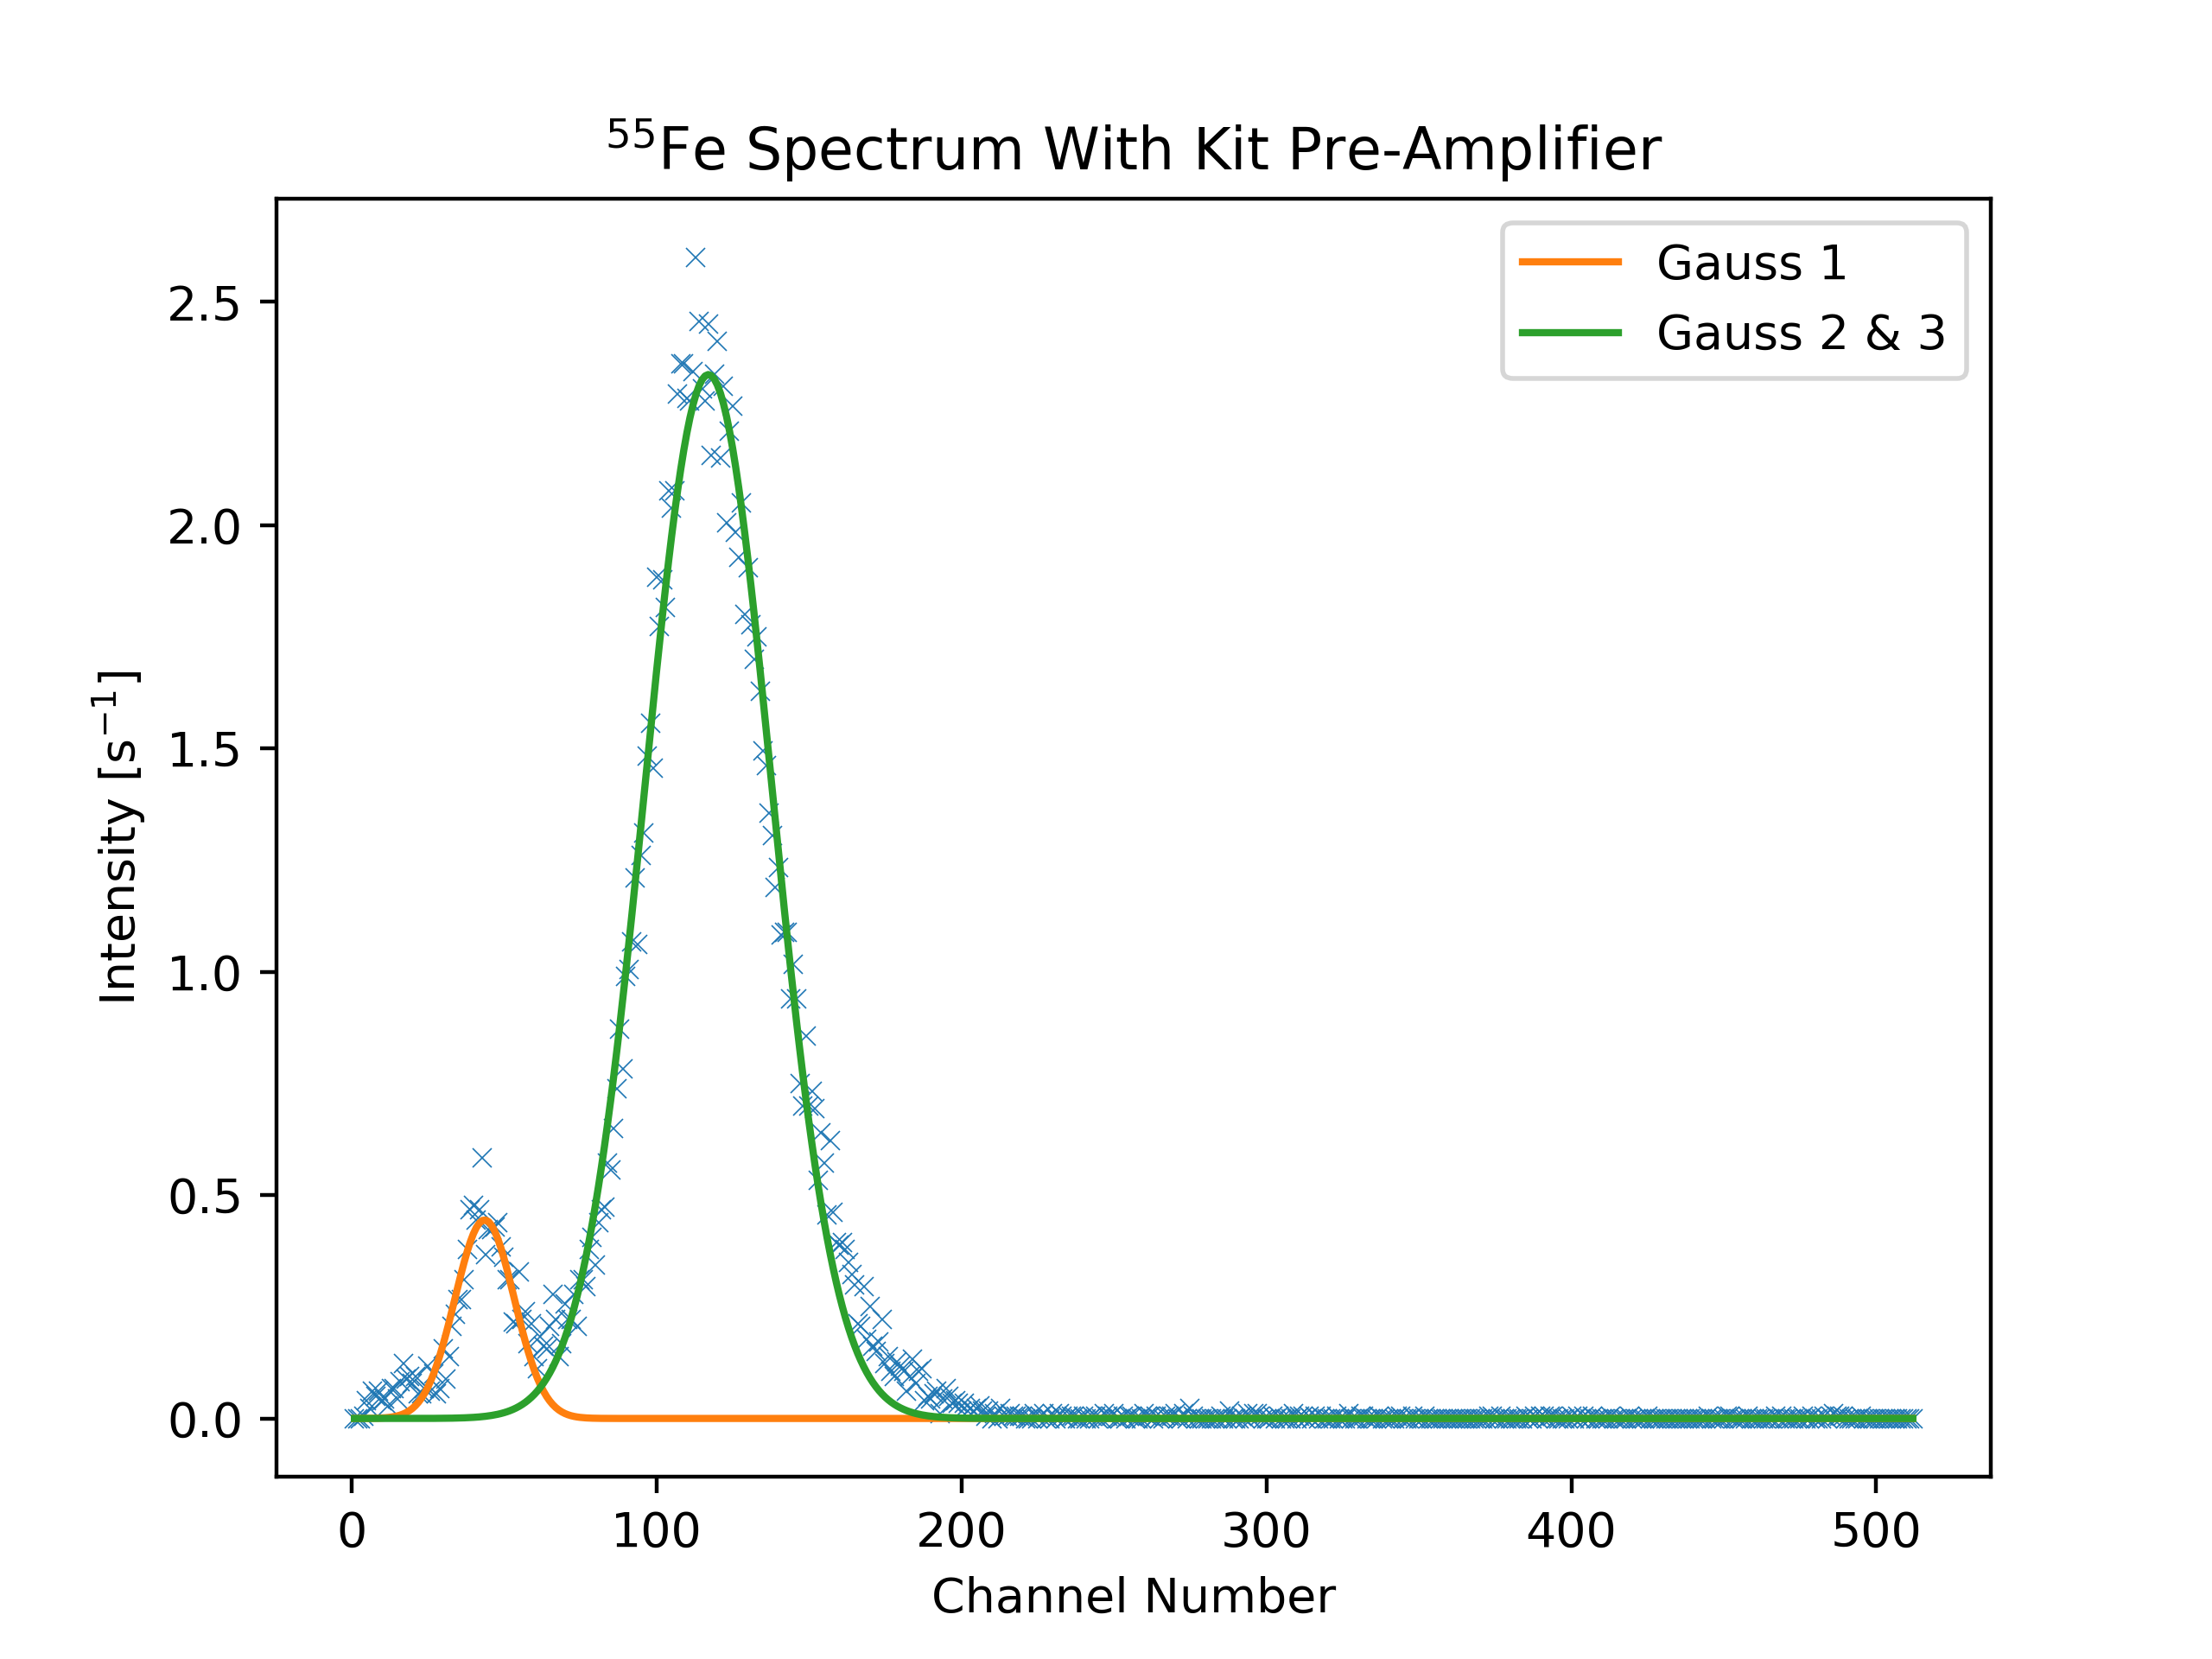
\includegraphics[width=\linewidth]{preamplifierSpectrum.png}
  \caption{Spectrum of \textsuperscript{55}Fe, measured using the kit preamplifier. The Gaussian curve fitted to the main photopeak was found to have a channel centre of (177.1$\pm$0.2) and a FWHM of (48.9$\pm$0.4). This means the peak has an energy resolution of (23.7$\pm$0.2)\%.}
  \label{fig:preampSpec}
\end{figure}